\documentclass[default,sn-mathphys,Numbered]{sn-jnl}

\usepackage{graphicx}
\usepackage{multirow}
\usepackage{amsmath,amssymb,amsfonts}
\usepackage{amsthm}
\usepackage{mathrsfs}
\usepackage[title]{appendix}
\usepackage{xcolor}
\usepackage{textcomp}
\usepackage{manyfoot}
\usepackage{booktabs}
\usepackage{algorithm}
\usepackage{algorithmicx}
\usepackage{algpseudocode}
\usepackage{url}

\raggedbottom

% >>> Replace with the real public repository URL before submission <<<
\newcommand{\repourl}{https://github.com/k8216/DE-RALBA-load-balancing-algorithm-experimental-setup}

\begin{document}

\title[Evaluating DE-RALBA under Steady and Bursty Workloads]{Evaluating DE-RALBA under Steady and Bursty Workloads: A Replication-and-Extension Study in CloudSim Plus}

\author[1]{\fnm{Anshal} \sur{}}\email{anshal.ug24@nsut.ac.in}
\equalcont{These authors contributed equally to this work.}
\author[1]{\fnm{Parna} \sur{Hembram}}\email{parna.hembram.ug24@nsut.ac.in}
\equalcont{These authors contributed equally to this work.}
\author*[1]{\fnm{Kunal} \sur{Kashyap}}\email{kunal.kashyap.ug24@nsut.ac.in}
\equalcont{These authors contributed equally to this work.}

\affil*[1]{\orgdiv{Department of Information Technology}, \orgname{Netaji Subhas University of Technology (NSUT)}, \orgaddress{\street{Sector-3, Dwarka}, \city{New Delhi}, \postcode{110078}, \country{India}}}

\abstract{Load balancing assigns incoming jobs (cloudlets) to virtual machines (VMs), and its quality depends on how jobs arrive. The Dynamic Enhanced Resource-Aware Load Balancing Algorithm (DE-RALBA) combines computation shares proportional to VM capacity, an Earliest Finish Time (EFT) step, runtime status updates, and reallocation of waiting cloudlets to idle VMs. Its original evaluation reports makespan and resource utilisation for batch workloads. This replication-and-extension study evaluates a corrected interpretation of DE-RALBA, a port of the authors' released code, a Big-First variant, and a variant without idle-VM reallocation under steady Poisson arrivals ($\rho = 0.5$ and $0.8$) and 10-second bursts of $4\times$, $20\times$, $60\times$ and $150\times$ the base rate. The baselines are Round Robin, EFT and Dynamic Max-Min, and the round-based algorithms are run with 1 s and 5 s scheduling intervals. Fifty heterogeneous VMs (52,500 MIPS in total) execute GoCJ job sizes using a discrete-event model of CloudSim Plus space-shared VMs, which agrees with CloudSim Plus 8.5.7 to within 0.16\% in makespan. Over 1,980 runs (30 paired seeds), Round Robin performs worst in every scenario. The corrected DE-RALBA variants match EFT and Dynamic Max-Min in makespan and recovery time but do not consistently outperform them: at $150\times$, EFT has the lowest mean response time (263.6 s against 269.4--282.6 s). The share step places almost no jobs except during intense bursts, which explains why DE-RALBA usually behaves like EFT. Idle-VM reallocation reduces mean response time in all twelve tested configurations without changing makespan. The port of the released code has a 2.5 times longer makespan at $150\times$ and does not recover in 28 of 30 seeds.}

\keywords{Cloud computing, Load balancing, DE-RALBA, Bursty workloads, CloudSim Plus, Replication study}

\maketitle

%======================================================================
\section{Introduction}\label{sec:intro}
%======================================================================

\subsection{Background}
Cloud computing provides computing resources such as processing power, storage, and memory through the internet, allowing users and organisations to run applications without maintaining their own physical infrastructure \cite{armbrust2010view, buyya2009cloud}. As the number of users and applications grows, incoming tasks (jobs, or cloudlets in simulation environments) must be assigned to available Virtual Machines (VMs) for execution. This process is known as load balancing \cite{shafiq2022review}.

Load balancing matters because an inefficient distribution of jobs can overload some VMs while others remain underutilised, increasing job completion time, response time, and overall system workload. An effective load-balancing algorithm should therefore consider both the processing capacity of VMs and the requirements of incoming jobs \cite{kumar2019comprehensive}.

\subsection{Research problem}
Job arrivals in cloud systems are not always uniform. Jobs may arrive at a steady rate or in sudden increases within a short period, known as workload bursts \cite{mi2008burstiness, bodik2010spikes}. An algorithm that performs well under a steady workload may not do so during a burst, when jobs wait longer for available VMs and the distribution of work across VMs may become less balanced.

Scheduling algorithms assign jobs using different criteria, such as VM availability, estimated completion time, job size, or VM processing capacity, and their behaviour can vary with workload conditions and with how often scheduling decisions are made. It is therefore important to evaluate load-balancing algorithms under both steady and bursty workloads rather than relying on a single workload condition.

\subsection{Research motivation}
The Dynamic Enhanced Resource-Aware Load Balancing Algorithm (DE-RALBA) \cite{hussain2025deralba} is a resource-aware scheduling approach designed for cloud computing environments. It uses information about VM processing capacity and job requirements to distribute workloads. Its scheduling process also includes status updates and attempts to reallocate waiting jobs when VMs become idle.

Although DE-RALBA has been evaluated in its original research, its behaviour under different burst intensities and scheduling intervals is worth examining further. This study therefore examines it under different workload conditions, investigates a Big-First modification that prioritises large jobs before share-based allocation, and examines the role of idle-VM reallocation.

Rather than proposing a new load-balancing algorithm, this work is a replication-and-extension study that evaluates a corrected interpretation of DE-RALBA under steady and bursty arrivals. It examines selected scheduling behaviours and implementation choices; it does not claim to validate the authors' released implementation or reproduce every detail of that implementation.

\subsection{Research objectives and questions}
The main objective of this research is to evaluate the behaviour of DE-RALBA under steady and bursty workloads in a simulated heterogeneous cloud. The study focuses on the following research questions:
\begin{itemize}
    \item \textbf{RQ1:} How does DE-RALBA perform under steady and bursty workloads compared with Round Robin, Earliest Finish Time (EFT), and Dynamic Max-Min scheduling algorithms?
    \item \textbf{RQ2:} How do the share-based allocation process, the Big-First modification, and idle-VM reallocation affect scheduling performance?
    \item \textbf{RQ3:} How does the scheduling interval affect the performance of DE-RALBA and other round-based scheduling approaches?
\end{itemize}
To answer these questions, the study evaluates scheduling performance using makespan, average resource utilisation ratio, average and 95th-percentile response time, load imbalance, and recovery time after a burst.

\subsection{Research contributions}
The main contributions of this study are as follows:
\begin{enumerate}
    \item Implementation and evaluation of a corrected interpretation of DE-RALBA, executed with a discrete-event model whose timing is validated against CloudSim Plus 8.5.7.
    \item Comparison with a port of the authors' released implementation \cite{rehman2025zenodo}.
    \item Evaluation of a Big-First modification that prioritises large jobs before share-based allocation.
    \item A paired ablation of idle-VM reallocation, using a Big-First variant with reallocation disabled.
    \item Evaluation under steady workloads and bursts with different arrival-rate multipliers.
    \item Analysis of 1 s and 5 s scheduling intervals and their effect on response time, workload distribution, and recovery.
\end{enumerate}
All source code, workload files, raw results and figure scripts are publicly available \cite{spikelb2026repo}.

The remainder of the paper is organised as follows. Section~\ref{sec:related} reviews related work, Section~\ref{sec:deralba} describes DE-RALBA and the evaluated variants, Section~\ref{sec:method} presents the experimental methodology, Section~\ref{sec:results} reports the results, Section~\ref{sec:discussion} discusses them, Section~\ref{sec:limits} lists the limitations, and Section~\ref{sec:conclusion} concludes the paper.

%======================================================================
\section{Background and Related Work}\label{sec:related}
%======================================================================

\subsection{Cloud computing and load balancing}
In a cloud environment, physical machines host VMs that execute user tasks, represented as cloudlets in CloudSim \cite{calheiros2011cloudsim} and CloudSim Plus \cite{silvafilho2017cloudsimplus}. Because VMs may have different processing capacities, load balancing aims to distribute jobs so that the workload is not concentrated on a few VMs while other resources remain underutilised \cite{manvi2014resource, singh2016survey}.

Load-balancing approaches are commonly static, using information available before execution, or dynamic, using updated information during execution \cite{shafiq2022review, arunarani2019task}. Dynamic scheduling adapts to changing workloads but requires monitoring and repeated decisions that add overhead.

\subsection{Resource-aware load balancing (RALBA)}
Resource-aware scheduling considers the processing capacity of available computing resources when assigning jobs. This is particularly important in heterogeneous cloud environments, where VMs may have different processing speeds. The Resource-Aware Load Balancing Algorithm (RALBA) \cite{hussain2018ralba} calculates the computation share of each resource and uses these shares to guide job allocation. It consists of two scheduling components:
\begin{itemize}
    \item \textbf{Fill scheduler:} assigns jobs to resources according to their computation shares. It gives preference to resources with higher computational capacity and continues allocating jobs while the share-based allocation condition is satisfied.
    \item \textbf{Spill scheduler:} assigns the remaining jobs using the Earliest Finish Time criterion, considering the expected completion time of jobs on available resources.
\end{itemize}
RALBA distributes work according to the computational capacity of resources rather than treating them equally. However, its share calculation is static and does not stay up to date as jobs are assigned and executed, which can affect allocation under changing workloads.

\subsection{Dynamic resource-aware load balancing (DRALBA)}
DRALBA \cite{nabi2021dralba} extends RALBA by incorporating runtime resource-status updates. According to Hussain et al.\ \cite{hussain2025deralba}, DRALBA consists of two schedulers: a dynamic-updater scheduler that updates the status of computing resources during execution, and a dynamic RALBA scheduler that performs a share-based phase followed by a phase that assigns larger jobs by earliest finish time. Runtime updates give DRALBA more recent information than RALBA, at the cost of higher computational complexity, and provide the foundation that DE-RALBA develops. OG-RADL \cite{nabi2021ogradl} follows a related resource-aware design for deadline-constrained cloud tasks.

\subsection{Other job scheduling algorithms}
\subsubsection{Min-Min and Max-Min}
Min-Min repeatedly assigns the pending job with the minimum completion time to the resource that provides it. It favours small jobs, so larger jobs may wait longer. Max-Min instead selects the job with the maximum minimum completion time and assigns it to the resource with the earliest finish for that job; it prioritises long jobs but may delay small ones \cite{braun2001comparison, elzeki2012improved}. Tabak et al.\ \cite{tabak2014improving} reduced the running time of these heuristics so that they scale to large task sets.

\subsubsection{Dynamic Max-Min}
Dynamic Max-Min \cite{mao2014maxmin} extends Max-Min by updating resource status after each scheduling iteration, so later decisions reflect the updated workload. It is included as a baseline that considers both completion time and changing availability, and it is also a baseline in the original DE-RALBA study \cite{hussain2025deralba}.

\subsubsection{Earliest Finish Time (EFT)}
Earliest Finish Time selects the resource expected to complete a particular job at the earliest time \cite{topcuoglu2002performance}. The estimated completion time depends on the resource's current ready time, the job's processing requirement, and the resource's processing capacity. For a job $i$ arriving at time $A_i$ and VM $j$,
\begin{equation}\label{eq:eftbase}
\mathit{EFT}_{ij} = \max(A_i, R_j) + \frac{\mathit{MI}_i}{\mathit{MIPS}_j},
\end{equation}
where $R_j$ is the ready time of VM $j$, $\mathit{MI}_i$ is the processing requirement of job $i$ in million instructions (MI), and $\mathit{MIPS}_j$ is the processing capacity of VM $j$ in million instructions per second. EFT is useful in heterogeneous environments because it considers both job requirements and VM capacity and load.

\subsubsection{Round Robin (RR)}
Round Robin assigns jobs to VMs in cyclic order. It is simple but ignores job size and VM capacity, so equal job counts can produce very unequal workloads on heterogeneous VMs \cite{ibrahim2020indepth}.

\subsubsection{Other dynamic and metaheuristic approaches}
Several other dynamic load balancers have been proposed, such as deadline- and elasticity-aware algorithms \cite{kumar2018deadline}, algorithms that minimise makespan while keeping resources busy \cite{kumar2020dynamic}, and priority-aware datacenter load balancing \cite{shafiq2021load}. PSSLB and PSSELB, which are baselines of the original DE-RALBA study, come from the reactive--proactive RePro-Active method \cite{alaei2018repro}. Metaheuristic schedulers, surveyed in \cite{zhan2015cloud, houssein2021metaheuristics, ghafari2022energy}, search over complete task batches; an example is the improved whale optimisation algorithm of Chen et al.\ \cite{chen2020woa}. These methods need many iterations per decision and are therefore not included here, since this study focuses on online decisions made every few seconds. Ibrahim et al.\ \cite{ibrahim2020indepth} showed empirically that the ranking of cloud schedulers depends strongly on the workload, which motivates evaluating DE-RALBA under workloads other than the one it was designed for.

\subsection{Dynamic Enhanced Resource-Aware Load Balancing (DE-RALBA)}
Hussain et al.\ \cite{hussain2025deralba} introduced DE-RALBA as an extension of the resource-aware scheduling approach. The algorithm aims to improve workload distribution by considering VM computational capacity and estimated job finish times while maintaining updated VM and job status information (Fig.~\ref{fig:arch}).

\begin{figure}[h]
\centering
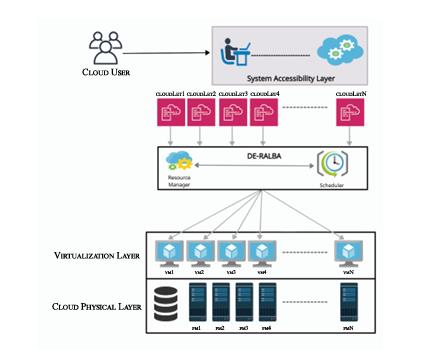
\includegraphics[width=0.62\textwidth]{figures_v2/fig1_deralba_architecture_hussain2025.png}
\caption{Overview of the DE-RALBA system architecture. Reproduced from Hussain et al.\ \cite{hussain2025deralba} (PeerJ Computer Science, CC BY 4.0).}\label{fig:arch}
\end{figure}

The reference study describes DE-RALBA as consisting of two sub-schedulers: (1) the DE-RALBA scheduler, which assigns jobs to VMs using computation shares and the EFT criterion, and (2) the Update-Scheduler, which maintains and updates VM and job execution information during runtime. The algorithm keeps a VM status table (computation shares, ready times, execution status and assigned jobs) and a job status table (job information and scheduling status). Figure~\ref{fig:flow} shows the scheduling flow.

\begin{figure}[h]
\centering
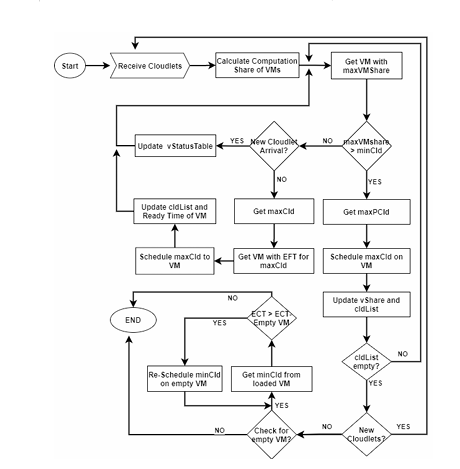
\includegraphics[width=0.62\textwidth]{figures_v2/fig2_deralba_flowchart_hussain2025.png}
\caption{Scheduling flow of DE-RALBA. Reproduced from Hussain et al.\ \cite{hussain2025deralba} (PeerJ Computer Science, CC BY 4.0).}\label{fig:flow}
\end{figure}

The scheduling process begins by selecting a VM with the largest available computation share. The scheduler identifies a suitable job for that VM, assigns the job, updates the VM status, and modifies its remaining share. This process continues while share-based allocation can be performed, and an EFT-based allocation process handles the remaining jobs. The original study evaluates the algorithm on GoCJ \cite{hussain2018gocj} and HCSP \cite{braun2000hcsp} workloads and compares it with DRALBA, PSSLB, PSSELB and Dynamic Max-Min, focusing on makespan and the Average Resource Utilisation Ratio (ARUR).

\subsection{Research gap and motivation}
Existing studies have examined resource-aware and dynamic scheduling, and the DE-RALBA study evaluates its algorithm against several approaches using simulation and workload datasets. However, behaviour can depend on arrival patterns and scheduling frequency, and steady-state performance may not explain behaviour under sudden bursts. This study therefore evaluates DE-RALBA and study-specific variants under steady and bursty workloads and two scheduling intervals. The contribution is an empirical evaluation, not a new algorithm or a validation of the published implementation. The present comparisons are limited to EFT, Dynamic Max-Min and Round Robin; DRALBA, PSSLB and PSSELB are not evaluated. The results therefore neither confirm nor refute the gains reported against those baselines by Hussain et al.\ \cite{hussain2025deralba}.

\subsection{Comparative summary of scheduling algorithms}
Table~\ref{tab:algos} summarises the main scheduling approaches and characteristics of the algorithms discussed in this section.

\begin{table}[h]
\caption{Comparison of cloud job scheduling algorithms (prepared from the descriptions in \cite{hussain2025deralba} and the cited sources)}\label{tab:algos}
\centering
\footnotesize
\begin{tabular}{p{1.7cm}p{3.6cm}p{2.9cm}p{3.2cm}}
\toprule
Algorithm & Main scheduling approach & Resource information & Main characteristic \\
\midrule
RALBA \cite{hussain2018ralba} & Fill and Spill schedulers: shares first, then EFT & Shares computed before scheduling & Capacity-aware but slow to adapt to runtime changes \\
DRALBA \cite{nabi2021dralba} & RALBA with runtime updates & Resource status updated during execution & Better adaptability through dynamic monitoring \\
DE-RALBA \cite{hussain2025deralba} & Shares, EFT step, status updates, idle-VM reallocation & VM and job status tables updated at runtime & Combines capacity-aware allocation with dynamic decisions \\
Dynamic Max-Min \cite{mao2014maxmin} & Largest minimum completion time first & Availability updated after each assignment & Prioritises long jobs \\
EFT \cite{topcuoglu2002performance} & Earliest estimated finish time & Ready time and capacity & Minimises each job's estimated completion \\
Round Robin & Cyclic order & Ignores job size and capacity & Simple, capacity-blind \\
\bottomrule
\end{tabular}
\end{table}

RALBA, DRALBA and DE-RALBA use resource-aware principles with increasing use of runtime information, Dynamic Max-Min and EFT rely on estimated completion times, and Round Robin uses simple cyclic assignment. These differences guide the selection of the algorithms evaluated here.

%======================================================================
\section{DE-RALBA Scheduling Process and Experimental Variants}\label{sec:deralba}
%======================================================================

\subsection{Overview}
DE-RALBA distributes cloudlets across VMs using VM processing capacity and estimated completion time \cite{hussain2025deralba}. Its scheduler assigns cloudlets, and its Update-Scheduler refreshes the VM status table, which holds each VM's capacity, computation share and ratio, ready time, executed, assigned and remaining MI, and last update time. The cloudlet status table holds each cloudlet's assigned VM, length and status. The scheduler also considers moving waiting cloudlets from loaded VMs to idle VMs.

\subsection{VM computation ratio and computation share}
For a system containing $m$ VMs, the computation ratio of VM $j$ is
\begin{equation}\label{eq:cr}
\mathit{CR}_j = \frac{\mathit{MIPS}_j}{\sum_{k=1}^{m} \mathit{MIPS}_k}.
\end{equation}
Let $\mathit{CLS}$ be the set of $n$ cloudlets available at the current scheduling decision and $\mathit{MI}_i$ the length of cloudlet $i$. The total workload and the computation share of VM $j$ are
\begin{equation}\label{eq:share}
W = \sum_{i=1}^{n} \mathit{MI}_i, \qquad \mathit{VMShare}_j = \mathit{CR}_j \cdot W .
\end{equation}

\subsection{Share-based cloudlet selection}
DE-RALBA selects cloudlets for the VM with the largest remaining computation share. For VM $j$ the eligible cloudlets and the selected cloudlet are
\begin{align}
\mathit{RPCloudlet}_j &= \{ c \in \mathit{CLS} \mid \mathit{MI}_c \le \mathit{VMShare}_j \}, \label{eq:rp}\\
\mathit{maxPCld}_j &= \arg\max_{c \in \mathit{RPCloudlet}_j} \mathit{MI}_c . \label{eq:maxp}
\end{align}
The scheduler also tracks the smallest and largest remaining cloudlets,
\begin{equation}\label{eq:minmax}
\mathit{minCld} = \min_{c \in \mathit{CLS}} \mathit{MI}_c, \qquad \mathit{maxCld} = \max_{c \in \mathit{CLS}} \mathit{MI}_c .
\end{equation}
Once a cloudlet is assigned it is removed from the unscheduled list, and the share of the selected VM is reduced:
\begin{equation}\label{eq:shareupd}
\mathit{VMShare}_j^{\text{new}} = \mathit{VMShare}_j^{\text{old}} - \mathit{MI}_i, \qquad
\mathit{maxVShare} = \max_{1 \le j \le m} \mathit{VMShare}_j .
\end{equation}

\subsection{EFT-based allocation of remaining cloudlets}
The share-based phase may leave cloudlets unassigned when every remaining cloudlet exceeds the selected VM's share. DE-RALBA then applies an EFT step: the largest remaining cloudlet is assigned to the VM expected to complete it earliest. The estimated completion time of cloudlet $i$ on VM $j$ is
\begin{equation}\label{eq:ct}
\mathit{CT}_{ij} = \frac{\mathit{MI}_i}{\mathit{MIPS}_j} + \mathit{VM\_CT}_j, \qquad
\mathit{VM\_CT}_j = \sum_{i=1}^{n} \frac{\mathit{MI}_i \cdot F[i,j]}{\mathit{MIPS}_j},
\end{equation}
where $F[i,j] = 1$ if cloudlet $i$ is assigned to VM $j$ and $0$ otherwise. The original paper prints the EFT value of a cloudlet as
\begin{equation}\label{eq:eftmax}
\mathit{Cld\_EFT}_i = \max_{1 \le j \le m} \mathit{CT}_{ij}.
\end{equation}
This contradicts the description of the algorithm as Earliest Finish Time, because selecting the maximum would identify the latest-finishing VM. This study uses the minimum-completion-time interpretation,
\begin{equation}\label{eq:eftmin}
\mathit{Cld\_EFT}_i = \min_{1 \le j \le m} \mathit{CT}_{ij},
\end{equation}
which follows the stated purpose of EFT. It is an interpretation of the paper's description, not an exact reproduction of the printed maximum operator.

\subsection{Update-Scheduler}
According to the original paper, the Update-Scheduler receives the VM status table and the current simulation time $t$ and updates the executed MI, remaining MI, ready time and last update time of each VM:
\begin{align}
\mathit{executedMI}_j &= \mathit{MIPS}_j \cdot t, \label{eq:exec}\\
\mathit{remMI}_j &= \mathit{totalAssignedMI}_j - \mathit{executedMI}_j, \label{eq:rem}\\
\mathit{readyTime}_j &= \mathit{readyTime}_j - (t - \mathit{lastUpdate}_j), \label{eq:ready}\\
\mathit{lastUpdate}_j &= t. \label{eq:last}
\end{align}
Equation~(\ref{eq:exec}) uses the absolute simulation time, whereas execution accounting needs the progress since the previous update (and only while the VM is busy). Equation~(\ref{eq:ready}) tracks the remaining busy time rather than the time at which the VM becomes available. The implementation therefore uses its own status accounting: executed MI is the sum of the finished cloudlets plus the executed part of the running one, and the ready time is the finish time of the last queued cloudlet (Section~\ref{sec:engine}).

\subsection{Idle-VM reallocation}
When a VM completes its assigned workload, the algorithm generates an empty-VM event. The scheduler identifies the idle VM and checks the cloudlets associated with loaded VMs. For each waiting candidate cloudlet $c$, it compares the expected finish time on the idle VM with the finish time on the VM currently holding it, and reassigns the cloudlet if the idle VM gives an earlier finish:
\begin{equation}\label{eq:realloc}
t_{\text{now}} + \frac{\mathit{MI}_c}{\mathit{MIPS}_{\text{empty}}} < F_c^{\text{loaded}},
\end{equation}
where $F_c^{\text{loaded}}$ is the projected finish time of $c$ on its current VM. In our implementation only cloudlets that have not yet started are moved. Loaded VMs are examined in decreasing order of ready time and their waiting cloudlets from smallest to largest, the fastest idle VM is served first, and the process repeats while an improving move exists.

\subsection{Performance model of the reference study}
The original paper evaluates scheduling performance with makespan and ARUR:
\begin{equation}\label{eq:mkarur}
\mathit{Makespan} = \max_{1 \le j \le m} \mathit{VM\_CT}_j, \qquad
\mathit{ARUR} = \frac{\frac{1}{m}\sum_{j=1}^{m} \mathit{VM\_CT}_j}{\mathit{Makespan}} .
\end{equation}
A lower makespan means the workload completes sooner. ARUR lies between 0 and 1, and higher values mean that VM completion times are closer to the makespan. Section~\ref{sec:metrics} states how the metrics are computed in this study.

\subsection{Scheduling process used in this study}
The implemented process follows the structure of the DE-RALBA paper, with explicit choices where its equations or pseudocode are ambiguous (Algorithm~\ref{alg:round}):
\begin{enumerate}
    \item At each decision point, the scheduler collects the cloudlets that arrived since the previous decision.
    \item It computes the VM computation ratios and shares from VM capacity and the total MI of these cloudlets (Eqs.~\ref{eq:cr}--\ref{eq:share}).
    \item It selects the VM with the largest remaining share, assigns the largest cloudlet that fits within that share, and deducts its MI from the share.
    \item If no cloudlet fits, the largest remaining cloudlet is assigned by minimum-completion-time EFT (Eq.~\ref{eq:eftmin}), using each VM's current backlog as its starting completion time.
    \item VM and cloudlet status are updated as execution progresses. When a VM becomes idle, waiting cloudlets are reallocated to it if this improves their expected completion time (Eq.~\ref{eq:realloc}).
\end{enumerate}

\begin{algorithm}[h]
\caption{One DE-RALBA round at decision time $t_k$ (corrected interpretation)}\label{alg:round}
\begin{algorithmic}[1]
\Require cloudlets $\mathit{CLS}$ that arrived since $t_{k-1}$; VM capacities $\mathit{MIPS}_j$; backlogs $b_j = \max(0, R_j - t_k)$; flag \textsc{BigFirst}
\State $W \gets \sum_{i \in \mathit{CLS}} \mathit{MI}_i$; \ $\mathit{VMShare}_j \gets \mathit{CR}_j W$; \ $C_j \gets b_j$ for all $j$
\If{\textsc{BigFirst}}
  \While{some unassigned $i$ has $\mathit{MI}_i > \max_j \mathit{VMShare}_j$}
    \State $i \gets$ the largest such cloudlet; \ $j^* \gets \arg\min_j (C_j + \mathit{MI}_i/\mathit{MIPS}_j)$
    \State assign $i \to j^*$; \ $C_{j^*} \mathrel{+}= \mathit{MI}_i/\mathit{MIPS}_{j^*}$; \ $\mathit{VMShare}_{j^*} \gets \max(0, \mathit{VMShare}_{j^*} - \mathit{MI}_i)$
  \EndWhile
\EndIf
\While{unassigned cloudlets remain}
  \State $j \gets \arg\max_j \mathit{VMShare}_j$; \ $i \gets$ largest unassigned cloudlet with $\mathit{MI}_i \le \mathit{VMShare}_j$
  \If{$i$ exists}
    \State assign $i \to j$; \ $\mathit{VMShare}_j \mathrel{-}= \mathit{MI}_i$; \ $C_j \mathrel{+}= \mathit{MI}_i/\mathit{MIPS}_j$ \Comment{share step}
  \Else
    \State $i \gets$ largest unassigned cloudlet; \ $j^* \gets \arg\min_j (C_j + \mathit{MI}_i/\mathit{MIPS}_j)$ \Comment{EFT step}
    \State assign $i \to j^*$; \ $C_{j^*} \mathrel{+}= \mathit{MI}_i/\mathit{MIPS}_{j^*}$
  \EndIf
\EndWhile
\State dispatch all cloudlets of the round at time $t_k$
\end{algorithmic}
\end{algorithm}

\subsection{Experimental algorithm variants}
\begin{itemize}
    \item \textbf{DE-RALBA-LIT}: a literal, corrected interpretation of the share-first process (Algorithm~\ref{alg:round} without Big-First). It is used to evaluate the main scheduling structure described in the paper.
    \item \textbf{DE-RALBA-BF}: adds a Big-First step. Before the normal share-based phase, cloudlets whose length exceeds the largest current VM share are assigned by EFT, largest first, and their lengths are deducted from the selected VMs' shares; the remaining cloudlets then go through the share-based phase. Big-First is an experimental modification introduced in this study, not an original feature of DE-RALBA.
    \item \textbf{DE-RALBA-BF-NOREB}: Big-First with idle-VM reallocation disabled. Comparing it with DE-RALBA-BF on the same seeds isolates the contribution of reallocation.
    \item \textbf{DE-RALBA-AUTHOR-ASIS}: follows the authors' released source code \cite{rehman2025zenodo}, ported to the execution engine used here. Differences from the corrected interpretation are treated as implementation differences, not as defects of the published algorithm. Notable differences in the released code are: the ready-time update $R_j \gets R_j + (\mathit{MI}_i/\mathit{MIPS}_j + R_j)$, which roughly doubles a busy VM's ready time at each assignment; a first-fit (rather than largest-fit) share search whose loop skips the last pending cloudlet; and a reallocation step that updates the status table without moving the cloudlet in the simulator.
\end{itemize}

\subsection{Baseline scheduling algorithms and decision intervals}
Round Robin, EFT and Dynamic Max-Min (Section~\ref{sec:related}) are the baselines. RR sends cloudlet $i$ to VM $i \bmod m$ on arrival. EFT assigns each cloudlet on arrival to the VM with the minimum estimated completion time (Eq.~\ref{eq:eftbase}). Dynamic Max-Min collects the cloudlets of a round and repeatedly selects the cloudlet whose earliest possible completion time is largest, assigns it to the VM that gives that completion time, and updates that VM's availability before the next selection.

The round-based algorithms make allocation decisions every 1 s or 5 s. A short interval considers waiting cloudlets more often, whereas a longer interval lets more accumulate in a batch but delays their scheduling. The interval is an experimental parameter, not a separate algorithm. The released-code variant is evaluated only at 1 s because its decisions are tied to a 1 s clock.

%======================================================================
\section{Experimental Methodology}\label{sec:method}
%======================================================================

\subsection{Simulation environment and execution engine}\label{sec:engine}
The experiments simulate a heterogeneous datacenter with 50 VMs. Each VM has a single processing element and the space-shared (FIFO) cloudlet scheduler of CloudSim Plus (\texttt{CloudletSchedulerSpaceShared}), so it runs one cloudlet at a time and queues the rest. The VM configuration is shown in Table~\ref{tab:vms}; the total VM capacity is 52,500 MIPS.

\begin{table}[h]
\caption{Virtual machine configuration}\label{tab:vms}
\centering
\footnotesize
\setlength{\tabcolsep}{3pt}
\begin{tabular}{lccccccccc}
\toprule
MIPS per VM & 100 & 500 & 550 & 1,000 & 1,250 & 1,500 & 1,750 & 2,000 & Total \\
Number of VMs & 7 & 7 & 6 & 6 & 6 & 6 & 6 & 6 & 50 \\
\bottomrule
\end{tabular}
\end{table}

Running 1,980 full CloudSim Plus simulations of 1,000 cloudlets each would be slow, so the cloudlet execution is computed by a discrete-event queue model (\texttt{QueueExec}) of these VMs. A cloudlet dispatched to VM $j$ at time $d_i$ starts at $S_i = \max(d_i, F_{\text{prev}})$, where $F_{\text{prev}}$ is the finish time of the previous cloudlet in that VM's queue, and finishes at $F_i = S_i + \mathit{MI}_i/\mathit{MIPS}_j$. To check this model, we executed four 100-cloudlet schedules both in \texttt{QueueExec} and in CloudSim Plus 8.5.7 (two with steady arrivals at $\rho = 0.5$, and two with a $20\times$ burst lasting 5 s from $t = 50$ s, which suits the shorter 100-cloudlet workload), with one host per VM, 512 MB RAM and 1,000 Mbps bandwidth per VM, and each cloudlet submitted with a delay equal to its dispatch time (Table~\ref{tab:valid}).

\begin{table}[h]
\caption{Agreement between the queue model and CloudSim Plus 8.5.7 on four 100-cloudlet schedules (times in seconds)}\label{tab:valid}
\centering
\scriptsize
\setlength{\tabcolsep}{3pt}
\begin{tabular}{lccccc}
\toprule
Schedule & Max $|\Delta S_i|$ & Max $|\Delta F_i|$ & Model makespan & CloudSim Plus makespan & Diff.\ \\
\midrule
RR, steady $\rho=0.5$ & 1.488 & 1.488 & 7,761.69 & 7,763.18 & 0.019\% \\
EFT, steady $\rho=0.5$ & 0.933 & 0.943 & 933.59 & 934.04 & 0.048\% \\
Dyn.\ Max-Min, 5 s, $20\times$ & 1.211 & 1.341 & 854.25 & 855.52 & 0.149\% \\
DE-RALBA-BF, 5 s, $20\times$ & 1.191 & 1.311 & 852.25 & 853.56 & 0.154\% \\
\bottomrule
\end{tabular}
\end{table}

The largest per-cloudlet difference is below 1.5 s and the largest makespan difference is 0.154\%. These small differences come from CloudSim Plus's minimum time between events (0.1 s), its VM creation at $t = 0.1$ s, and its integer cloudlet lengths. Host-level effects such as network delays are not modelled (Section~\ref{sec:limits}).

\subsection{Workload dataset}
The experiments use cloudlet lengths from the GoCJ dataset \cite{hussain2018gocj, hussain2018gocjdata}, which provides cloudlet processing requirements in MI. A 100-cloudlet GoCJ instance is used as the pool of lengths: minimum 15,000 MI, mean 135,095 MI, maximum 900,000 MI. Each run contains 1,000 cloudlets, drawn by shuffling the pool for each seed and reshuffling it each time it is exhausted. For a given seed, all algorithms receive the same cloudlets and arrival times.

\subsection{Workload arrival model}
Arrivals follow a Poisson process whose rate is determined by the offered-load parameter $\rho$, the total VM capacity $C_{\text{total}}$, and the mean cloudlet length $\mathit{MI}_{\text{mean}}$:
\begin{equation}\label{eq:lambda}
\lambda = \frac{\rho \cdot C_{\text{total}}}{\mathit{MI}_{\text{mean}}} = \frac{\rho \times 52{,}500}{135{,}095}\ \text{jobs/s},
\end{equation}
which gives $\lambda \approx 0.194$ jobs/s for $\rho = 0.5$. Under this model the number of arrivals $N(\Delta t)$ during an interval of duration $\Delta t$ follows a Poisson distribution:
\begin{equation}\label{eq:poisson}
P\left(N(\Delta t) = k\right) = \frac{(\lambda \Delta t)^k e^{-\lambda \Delta t}}{k!}, \qquad k = 0, 1, 2, \dots
\end{equation}

\subsection{Steady and bursty workload scenarios}
The steady scenarios use $\rho = 0.5$ and $\rho = 0.8$. The burst scenarios use $\rho = 0.5$ as the base load and multiply the arrival rate by a factor $b$ for 10 s starting at $t = 1{,}000$ s:
\begin{equation}\label{eq:burst}
\lambda(t) = \begin{cases} b\,\lambda, & 1000 \le t < 1010 \text{ s},\\ \lambda, & \text{otherwise}, \end{cases}
\end{equation}
with $b \in \{4, 20, 60, 150\}$ (Table~\ref{tab:scen}). The number of cloudlets arriving during a burst is random; in the $150\times$ scenario an average of 289.4 cloudlets arrived during the 10-second burst.

\begin{table}[h]
\caption{Workload scenarios}\label{tab:scen}
\centering
\begin{tabular}{lccc}
\toprule
Scenario & Baseline offered load & Burst multiplier & Burst duration \\
\midrule
Steady workload 1 & 0.5 & none & --- \\
Steady workload 2 & 0.8 & none & --- \\
Burst workload 1 & 0.5 & $4\times$ & 10 s \\
Burst workload 2 & 0.5 & $20\times$ & 10 s \\
Burst workload 3 & 0.5 & $60\times$ & 10 s \\
Burst workload 4 & 0.5 & $150\times$ & 10 s \\
\bottomrule
\end{tabular}
\end{table}

\subsection{Random seeds and experiment matrix}
Each scenario is evaluated with 30 random seeds. The same seed is used across algorithms, with separate random-number streams for cloudlet sizes and Poisson arrivals, so that algorithms receive identical workloads and paired comparisons are possible. The experiment matrix contains 11 algorithm configurations: RR; EFT; Dynamic Max-Min, DE-RALBA-LIT, DE-RALBA-BF and DE-RALBA-BF-NOREB, each with 1 s and 5 s intervals; and DE-RALBA-AUTHOR-ASIS with 1 s. Six scenarios, 30 seeds and 11 configurations give $6 \times 30 \times 11 = 1{,}980$ runs. (The public results file also contains additional runs with 30 s intervals and a backlog-aware share variant, which are not analysed in this paper.)

\subsection{Performance metrics}\label{sec:metrics}
\begin{itemize}
    \item \textbf{Makespan.} In the tables, makespan is the finish time of the last cloudlet, $\max_i F_i$. Figure~\ref{fig:mkarur} additionally uses the paper definition of Eq.~(\ref{eq:mkarur}), where $\mathit{VM\_CT}_j$ is the total busy time of VM $j$. The two definitions are close for all corrected algorithms.
    \item \textbf{ARUR} is computed with Eq.~(\ref{eq:mkarur}) using VM busy times. It measures how evenly busy time is spread and is not a time-averaged CPU utilisation.
    \item \textbf{Response time} of cloudlet $i$ is $\mathit{RT}_i = F_i - A_i$. We report the mean over all cloudlets, the 95th percentile (p95) and the maximum.
    \item \textbf{Load imbalance} is $I = B_{\max}/B_{\text{mean}}$, where $B_j$ is the busy time of VM $j$. A value of 1 means that all VMs are equally busy; note that $I = 1/\mathit{ARUR}$.
    \item \textbf{Recovery time} is measured from the end of the burst ($t = 1{,}010$ s). Let $X(t)$ be the total queued work in the cluster (in seconds), and $\bar{X}$ and $\sigma$ its mean and standard deviation during $500 \le t < 1000$ s. The system has recovered when $X(t)$ stays at or below $\bar{X} + \max(0.25\bar{X}, 2\sigma) + 1$ s for 60 consecutive seconds. If this has not happened by the last arrival, the run is \emph{censored} and its recovery value is a lower bound.
\end{itemize}

\subsection{Statistical analysis}
Results are aggregated over the 30 seeds for each configuration and scenario. For a metric $X$ with sample mean $\bar{X}$ and standard deviation $s$ over $r = 30$ runs, the 95\% confidence interval is
\begin{equation}\label{eq:ci}
\bar{X} \pm t_{0.975,\,r-1} \frac{s}{\sqrt{r}}, \qquad t_{0.975,\,29} = 2.045 .
\end{equation}
Because the same seeds are used across algorithms, we also compute paired per-seed differences $\Delta_s = X_s^{(A)} - X_s^{(B)}$ and report their means with 95\% confidence intervals.

%======================================================================
\section{Experimental Results}\label{sec:results}
%======================================================================

\subsection{Overview}
This section presents the results for six workload scenarios over 1,980 runs. Figure~\ref{fig:mkarur} gives an overview of makespan and ARUR. In this and the following figures, ``EFT'' denotes EFT with immediate dispatch, ``Max-Min'' Dynamic Max-Min, ``big-first'' DE-RALBA-BF, and ``as-printed'' DE-RALBA-AUTHOR-ASIS. Markers show means over the 30 seeds and error bars show 95\% confidence intervals.

\begin{figure}[h]
\centering
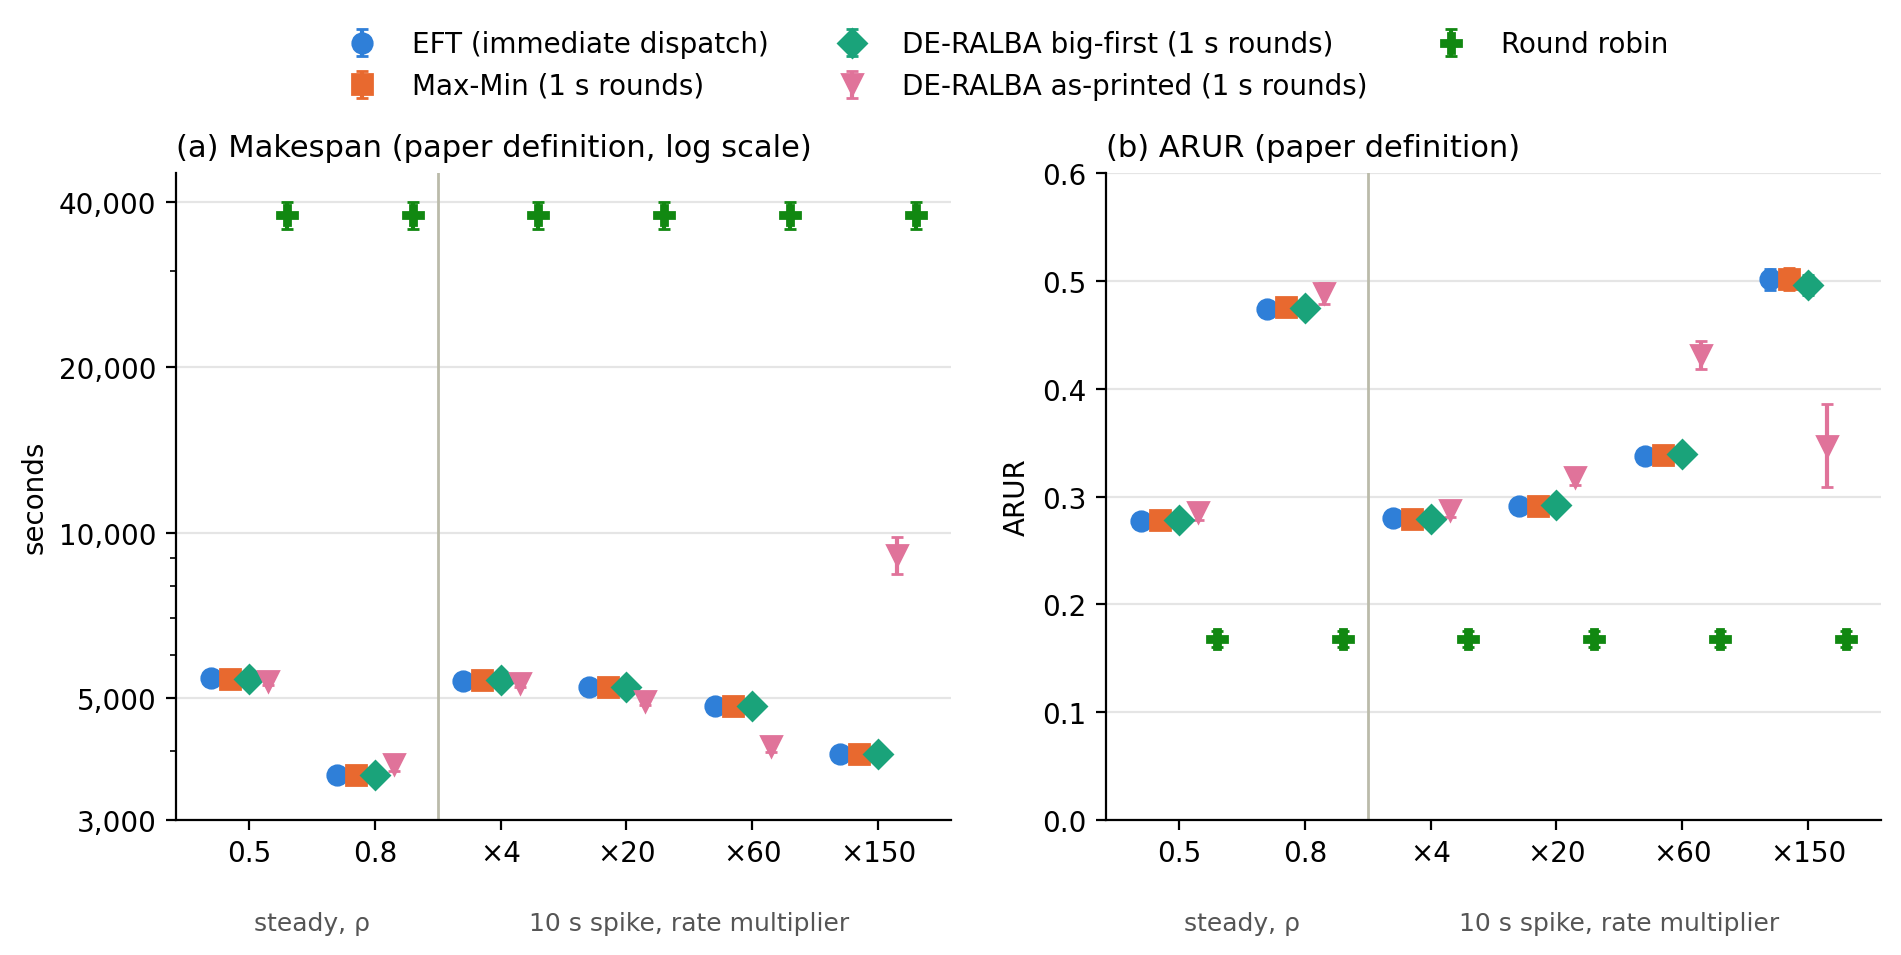
\includegraphics[width=\textwidth]{figures_v2/fig3_makespan_arur.png}
\caption{Makespan (a, log scale) and ARUR (b), computed with the definitions of the original paper (Eq.~\ref{eq:mkarur}), for the two steady and four burst scenarios.}\label{fig:mkarur}
\end{figure}

Round Robin is clearly separated from all other algorithms, with makespan near 38,000 s and ARUR near 0.17 in every scenario. EFT, Dynamic Max-Min and DE-RALBA big-first are practically indistinguishable in both metrics. DE-RALBA as-printed departs clearly in makespan only under the $150\times$ burst, where it is more than twice that of the other algorithms; its ARUR is higher in the $20\times$ and $60\times$ bursts but lower at $150\times$, so ARUR must be read together with other metrics. Differences between scenarios largely reflect the arrival process, so algorithms should be compared within a scenario.

\subsection{Performance under steady workloads}
Tables~\ref{tab:rho05} and~\ref{tab:rho08} present the results for the steady workloads. Values are means over 30 seeds with 95\% confidence-interval half-widths.

\begin{table}[h]
\caption{Results under the steady workload with $\rho = 0.5$ (mean $\pm$ 95\% CI half-width, 30 seeds). LIT, BF, BF-NOREB and AUTHOR-ASIS denote the DE-RALBA variants.}\label{tab:rho05}
\centering
\fontsize{6.6pt}{8pt}\selectfont
\setlength{\tabcolsep}{2pt}
\begin{tabular}{lccccc}
\toprule
Algorithm & Makespan (s) & ARUR & Mean RT (s) & p95 RT (s) & Imbalance \\
\midrule
RR & $37{,}854.3 \pm 2{,}164.9$ & $0.168 \pm 0.007$ & $1{,}876.5 \pm 54.2$ & $13{,}737.2 \pm 616.3$ & $6.05 \pm 0.29$ \\
EFT & $5{,}498.6 \pm 52.0$ & $0.277 \pm 0.003$ & $79.6 \pm 0.3$ & $325.3 \pm 3.2$ & $3.61 \pm 0.04$ \\
Dyn.\ Max-Min, 1 s & $5{,}495.6 \pm 51.6$ & $0.278 \pm 0.003$ & $79.9 \pm 0.2$ & $324.1 \pm 3.1$ & $3.60 \pm 0.04$ \\
Dyn.\ Max-Min, 5 s & $5{,}494.9 \pm 52.9$ & $0.278 \pm 0.003$ & $81.6 \pm 0.2$ & $325.4 \pm 3.1$ & $3.60 \pm 0.04$ \\
LIT, 1 s & $5{,}495.7 \pm 51.7$ & $0.278 \pm 0.003$ & $80.0 \pm 0.2$ & $324.2 \pm 3.2$ & $3.60 \pm 0.04$ \\
LIT, 5 s & $5{,}495.2 \pm 53.1$ & $0.278 \pm 0.003$ & $81.7 \pm 0.2$ & $325.6 \pm 3.0$ & $3.61 \pm 0.04$ \\
BF, 1 s & $5{,}495.7 \pm 51.7$ & $0.278 \pm 0.003$ & $80.0 \pm 0.2$ & $324.2 \pm 3.2$ & $3.60 \pm 0.04$ \\
BF, 5 s & $5{,}496.4 \pm 52.6$ & $0.278 \pm 0.003$ & $81.7 \pm 0.2$ & $325.4 \pm 3.0$ & $3.61 \pm 0.04$ \\
BF-NOREB, 1 s & $5{,}495.3 \pm 51.8$ & $0.278 \pm 0.003$ & $80.0 \pm 0.2$ & $325.1 \pm 4.0$ & $3.60 \pm 0.04$ \\
BF-NOREB, 5 s & $5{,}495.6 \pm 52.9$ & $0.278 \pm 0.003$ & $82.1 \pm 0.3$ & $334.5 \pm 5.8$ & $3.60 \pm 0.04$ \\
AUTHOR-ASIS, 1 s & $6{,}223.1 \pm 271.4$ & $0.285 \pm 0.007$ & $214.0 \pm 23.5$ & $676.0 \pm 105.8$ & $3.52 \pm 0.08$ \\
\bottomrule
\end{tabular}
\end{table}

RR is substantially worse than the other algorithms (makespan about 37,854 s against about 5,495 s). It sends 14\% of the cloudlets to the seven 100-MIPS VMs, which provide only 1.3\% of the capacity, so these VMs build long queues. EFT, Dynamic Max-Min, DE-RALBA-LIT and DE-RALBA-BF give very similar makespan, ARUR and imbalance, and the 5 s configurations have average response times about 1.7 s higher than the 1 s ones because cloudlets wait for the next decision. DE-RALBA-AUTHOR-ASIS has a 13\% higher makespan and 2.7 times the average response time of EFT; its slightly higher ARUR does not correspond to better response times. Overall, the corrected variants perform like EFT and Dynamic Max-Min here, and Big-First gives no clear improvement.

\begin{table}[h]
\caption{Results under the steady workload with $\rho = 0.8$ (mean $\pm$ 95\% CI half-width, 30 seeds). LIT, BF, BF-NOREB and AUTHOR-ASIS denote the DE-RALBA variants.}\label{tab:rho08}
\centering
\fontsize{6.6pt}{8pt}\selectfont
\setlength{\tabcolsep}{2pt}
\begin{tabular}{lccccc}
\toprule
Algorithm & Makespan (s) & ARUR & Mean RT (s) & p95 RT (s) & Imbalance \\
\midrule
RR & $37{,}844.7 \pm 2{,}165.9$ & $0.168 \pm 0.007$ & $2{,}157.2 \pm 52.9$ & $14{,}967.8 \pm 603.6$ & $6.05 \pm 0.29$ \\
EFT & $3{,}651.5 \pm 33.4$ & $0.474 \pm 0.006$ & $103.9 \pm 1.9$ & $371.8 \pm 3.9$ & $2.11 \pm 0.03$ \\
Dyn.\ Max-Min, 1 s & $3{,}641.3 \pm 32.2$ & $0.475 \pm 0.006$ & $104.1 \pm 1.9$ & $371.2 \pm 4.0$ & $2.11 \pm 0.03$ \\
Dyn.\ Max-Min, 5 s & $3{,}653.4 \pm 34.5$ & $0.475 \pm 0.006$ & $105.1 \pm 1.9$ & $370.6 \pm 3.8$ & $2.11 \pm 0.03$ \\
LIT, 1 s & $3{,}648.2 \pm 31.3$ & $0.475 \pm 0.006$ & $104.2 \pm 1.9$ & $370.8 \pm 4.1$ & $2.11 \pm 0.03$ \\
LIT, 5 s & $3{,}647.7 \pm 33.8$ & $0.475 \pm 0.006$ & $105.2 \pm 1.9$ & $369.6 \pm 3.8$ & $2.11 \pm 0.03$ \\
BF, 1 s & $3{,}648.2 \pm 31.3$ & $0.475 \pm 0.006$ & $104.2 \pm 1.9$ & $370.8 \pm 4.1$ & $2.11 \pm 0.03$ \\
BF, 5 s & $3{,}648.6 \pm 34.1$ & $0.475 \pm 0.007$ & $105.3 \pm 1.9$ & $370.3 \pm 3.8$ & $2.11 \pm 0.03$ \\
BF-NOREB, 1 s & $3{,}647.6 \pm 31.9$ & $0.475 \pm 0.006$ & $104.4 \pm 1.9$ & $371.7 \pm 4.3$ & $2.11 \pm 0.03$ \\
BF-NOREB, 5 s & $3{,}648.7 \pm 30.6$ & $0.476 \pm 0.006$ & $106.5 \pm 1.8$ & $374.5 \pm 4.4$ & $2.10 \pm 0.03$ \\
AUTHOR-ASIS, 1 s & $4{,}534.8 \pm 196.1$ & $0.488 \pm 0.010$ & $195.0 \pm 14.4$ & $600.0 \pm 65.7$ & $2.05 \pm 0.04$ \\
\bottomrule
\end{tabular}
\end{table}

At $\rho = 0.8$ the picture is the same: the corrected DE-RALBA variants, EFT and Dynamic Max-Min agree within the confidence intervals on every metric, and DE-RALBA-AUTHOR-ASIS has a higher makespan (about 4,535 s) and nearly twice the average response time of EFT.

\subsection{Performance under burst workloads}
\subsubsection{Bursts of $4\times$, $20\times$ and $60\times$}
Under the $4\times$, $20\times$ and $60\times$ bursts, the mean makespan of EFT is about 5,461, 5,304 and 4,901 s, and DE-RALBA-LIT and DE-RALBA-BF are within about 4 s of EFT in each case. DE-RALBA-AUTHOR-ASIS has a higher makespan (about 6,023, 5,804 and 5,162 s) and a higher ARUR (about 0.288, 0.318 and 0.431, against about 0.28, 0.29 and 0.34 for the other algorithms).

\subsubsection{Burst of $150\times$}
The $150\times$ burst is the most intense tested increase in arrival rate (Table~\ref{tab:x150}).

\begin{table}[h]
\caption{Results under the $150\times$ burst (mean $\pm$ 95\% CI half-width, 30 seeds). Cens.\ = number of seeds not recovered by the last arrival; for those seeds the recovery value is a lower bound. LIT, BF, BF-NOREB and AUTHOR-ASIS denote the DE-RALBA variants.}\label{tab:x150}
\centering
\fontsize{6.0pt}{7.4pt}\selectfont
\setlength{\tabcolsep}{2.6pt}
\begin{tabular}{lccccccc}
\toprule
Algorithm & Makespan (s) & ARUR & Mean RT (s) & p95 RT (s) & Max RT (s) & Recovery (s) & Cens. \\
\midrule
RR & $37{,}854.3\pm 2{,}164.9$ & $0.168\pm 0.007$ & $2{,}269.2\pm 52.8$ & $15{,}167.1\pm 613.0$ & $34{,}409.9\pm 2{,}144.8$ & $2{,}668.0\pm 48.1$ & 30/30 \\
EFT & $4{,}000.6\pm 51.8$ & $0.501\pm 0.010$ & $263.6\pm 8.8$ & $705.1\pm 15.8$ & $1{,}134.0\pm 29.5$ & $1{,}556.8\pm 53.9$ & 0/30 \\
Dyn.\ Max-Min, 1 s & $4{,}004.4\pm 52.5$ & $0.502\pm 0.010$ & $271.8\pm 9.3$ & $725.4\pm 17.0$ & $1{,}118.9\pm 29.0$ & $1{,}556.6\pm 53.6$ & 0/30 \\
Dyn.\ Max-Min, 5 s & $4{,}005.6\pm 51.8$ & $0.505\pm 0.009$ & $292.3\pm 10.0$ & $776.8\pm 20.0$ & $1{,}112.3\pm 29.5$ & $1{,}553.2\pm 53.3$ & 0/30 \\
LIT, 1 s & $4{,}004.3\pm 53.0$ & $0.497\pm 0.010$ & $282.6\pm 9.3$ & $836.8\pm 17.6$ & $1{,}159.8\pm 33.0$ & $1{,}551.5\pm 48.6$ & 0/30 \\
LIT, 5 s & $4{,}003.3\pm 52.4$ & $0.502\pm 0.009$ & $269.4\pm 10.0$ & $722.5\pm 20.9$ & $1{,}210.0\pm 24.3$ & $1{,}557.4\pm 54.0$ & 0/30 \\
BF, 1 s & $4{,}002.7\pm 51.8$ & $0.496\pm 0.010$ & $281.5\pm 9.1$ & $826.3\pm 18.7$ & $1{,}153.7\pm 29.6$ & $1{,}551.8\pm 48.4$ & 0/30 \\
BF, 5 s & $4{,}006.5\pm 51.9$ & $0.503\pm 0.010$ & $278.4\pm 10.1$ & $734.2\pm 20.3$ & $1{,}153.8\pm 24.9$ & $1{,}554.5\pm 53.3$ & 0/30 \\
BF-NOREB, 1 s & $4{,}001.3\pm 52.5$ & $0.491\pm 0.010$ & $282.4\pm 9.1$ & $832.5\pm 18.5$ & $1{,}159.7\pm 29.4$ & $1{,}561.6\pm 52.4$ & 0/30 \\
BF-NOREB, 5 s & $4{,}001.9\pm 53.0$ & $0.502\pm 0.010$ & $278.9\pm 10.1$ & $734.1\pm 20.4$ & $1{,}156.7\pm 24.7$ & $1{,}556.1\pm 53.7$ & 0/30 \\
AUTHOR-ASIS, 1 s & $10{,}142.8\pm 691.3$ & $0.347\pm 0.039$ & $444.3\pm 7.8$ & $1{,}199.7\pm 14.3$ & $8{,}036.3\pm 681.5$ & $2{,}661.6\pm 49.0$ & 28/30 \\
\bottomrule
\end{tabular}
\end{table}

RR is far worse than the other algorithms (makespan about 37,854 s, average response time about 2,269 s). EFT, Dynamic Max-Min, DE-RALBA-LIT and DE-RALBA-BF have similar makespan (close to 4,000 s) and recovery time (about 1,551--1,562 s). The corrected DE-RALBA variants have higher average response times than EFT (269.4--282.6 s against 263.6 s). DE-RALBA-LIT with 5 s rounds has the lowest average and p95 response time among the DE-RALBA configurations, while EFT has the lowest of all algorithms. DE-RALBA-AUTHOR-ASIS has a mean makespan of about 10,143 s, 2.5 times that of the corrected variants, an average response time of about 444 s, and a maximum response time of about 8,036 s. The corrected variants therefore keep makespan and recovery close to EFT and Dynamic Max-Min under the most intense burst, but they do not consistently outperform these baselines on response time.

\subsubsection{Response time across scenarios}
Figure~\ref{fig:rt} shows the mean and p95 response time of EFT, Dynamic Max-Min (1 s) and DE-RALBA big-first with 1 s and 5 s rounds in all six scenarios. DE-RALBA as-printed is omitted because its response times are much higher (Tables~\ref{tab:rho05}--\ref{tab:x150}).

\begin{figure}[h]
\centering
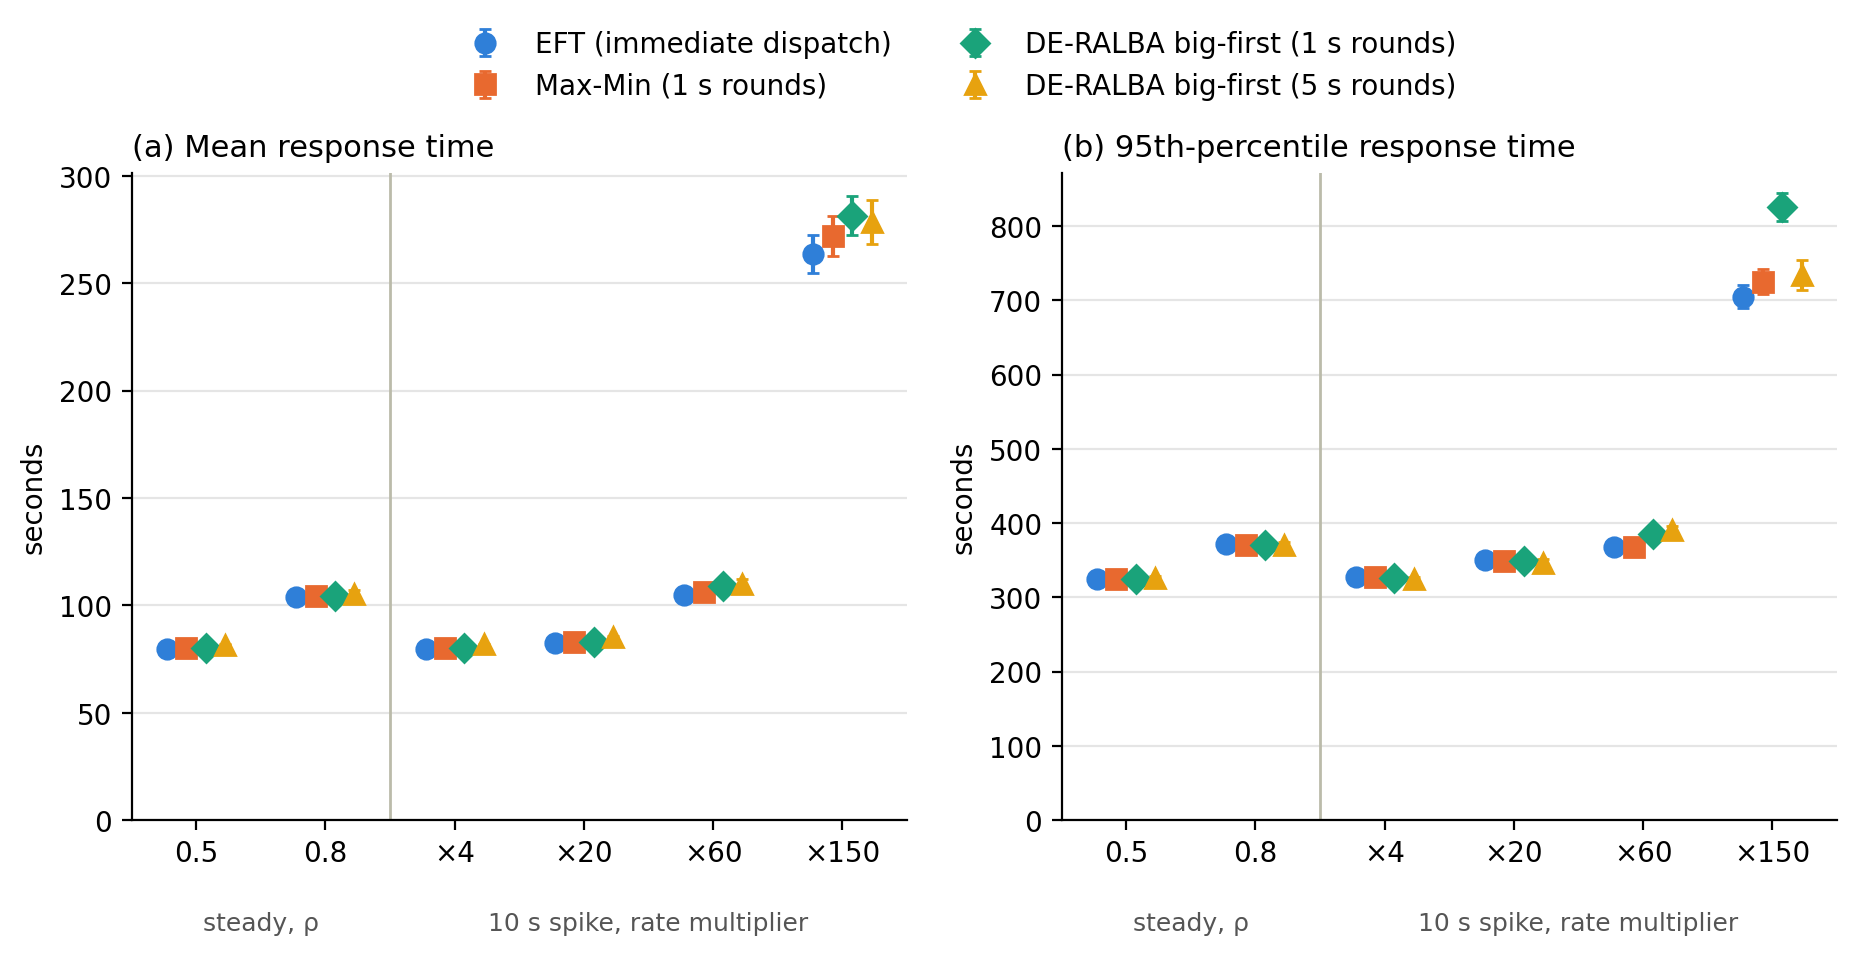
\includegraphics[width=\textwidth]{figures_v2/fig4_response_time.png}
\caption{Mean (a) and 95th-percentile (b) response time under steady and burst workloads.}\label{fig:rt}
\end{figure}

Under both steady workloads and the $4\times$ and $20\times$ bursts, the four configurations are close; differences remain small at $60\times$. A clearer separation appears at $150\times$, where the plotted configurations have mean response times of about 264--282 s and p95 values from about 705 to 826 s.

\subsubsection{Paired differences from the baselines}
Because every algorithm receives the same workload for a given seed, Fig.~\ref{fig:paired} reports paired per-seed differences between DE-RALBA big-first (BF) and the baselines (positive values mean DE-RALBA is slower): BF (1 s) minus EFT, BF (1 s) minus Max-Min (1 s), and BF (5 s) minus Max-Min (5 s).

\begin{figure}[h]
\centering
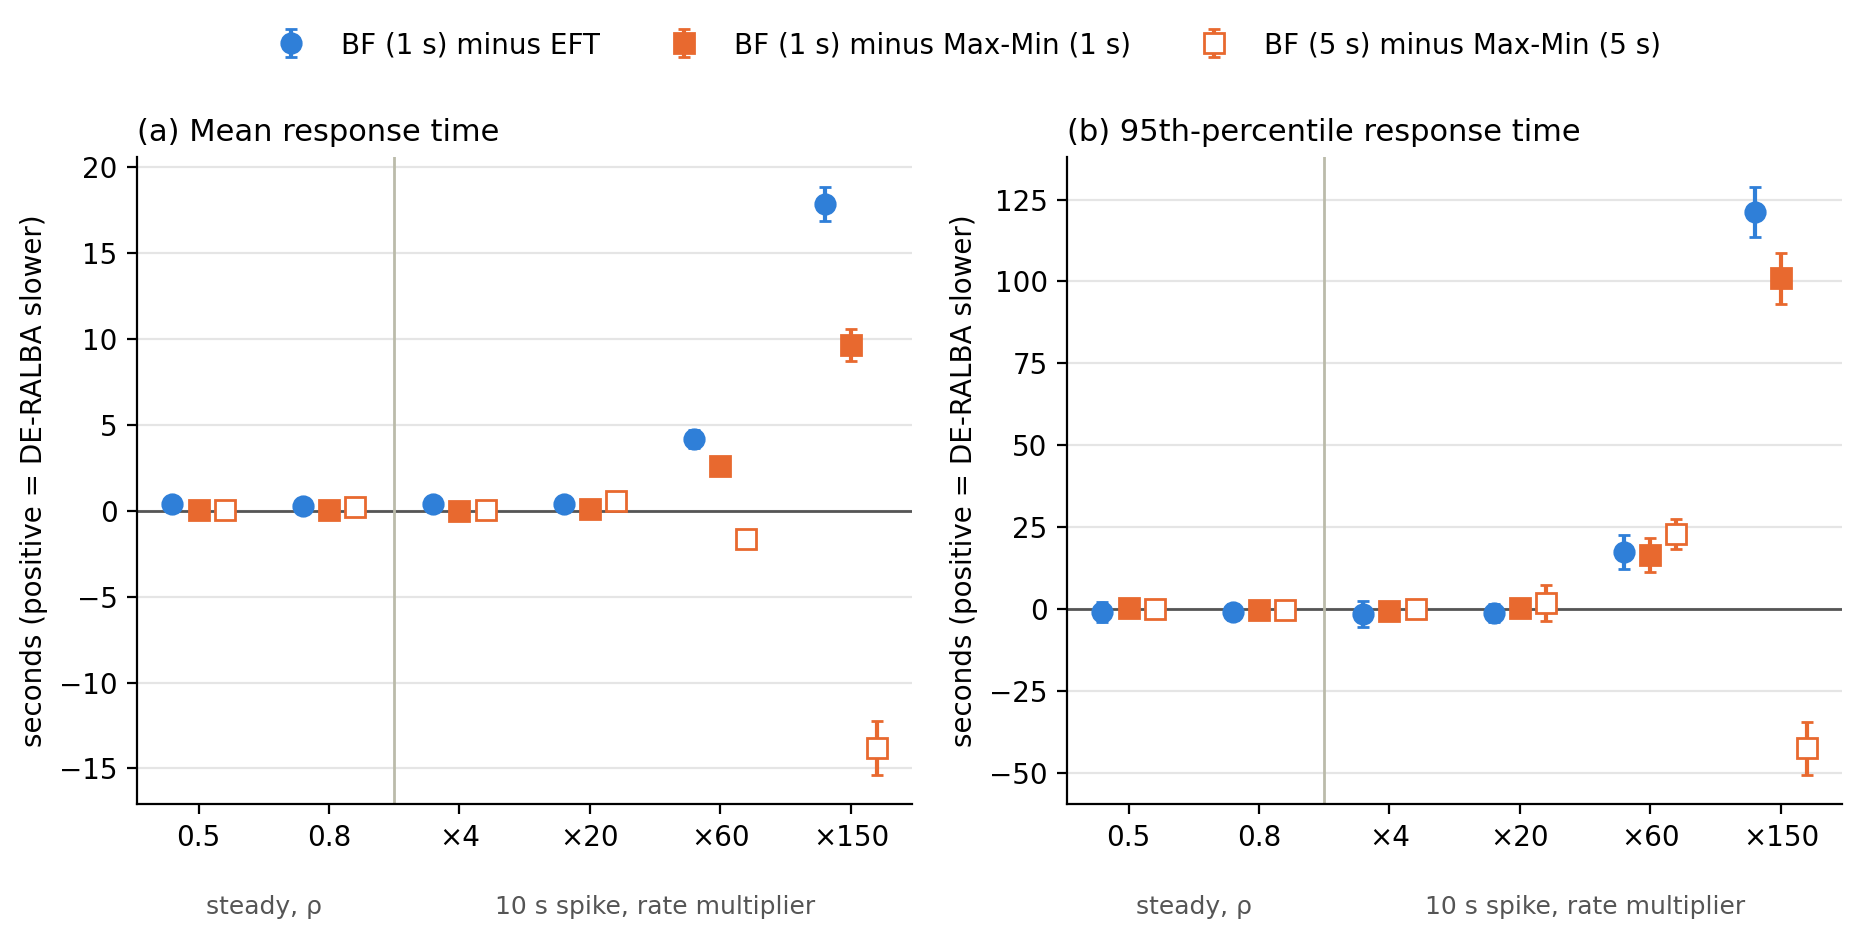
\includegraphics[width=\textwidth]{figures_v2/fig5_paired_vs_baselines.png}
\caption{Paired per-seed differences in mean (a) and 95th-percentile (b) response time between DE-RALBA big-first (BF) and the baselines, with 95\% confidence intervals. Positive values indicate that DE-RALBA is slower.}\label{fig:paired}
\end{figure}

Differences are close to zero in both steady scenarios and at $4\times$ and $20\times$. At $60\times$, the p95 differences are positive for all three comparisons (about 16--23 s). At $150\times$, big-first with 1 s rounds is about 18 s above EFT and 10 s above Max-Min in mean response time, and about 121 s and 101 s higher at the 95th percentile. The 5 s comparison goes the other way: big-first is about 14 s faster than Max-Min in mean and about 43 s faster at the 95th percentile. These selected comparisons are not adjusted for multiple testing and should be read as exploratory; the pattern also depends on the scheduling interval.

\subsubsection{Recovery after the burst}
Figure~\ref{fig:recovery} shows the recovery time after the end of the 10-second burst.

\begin{figure}[h]
\centering
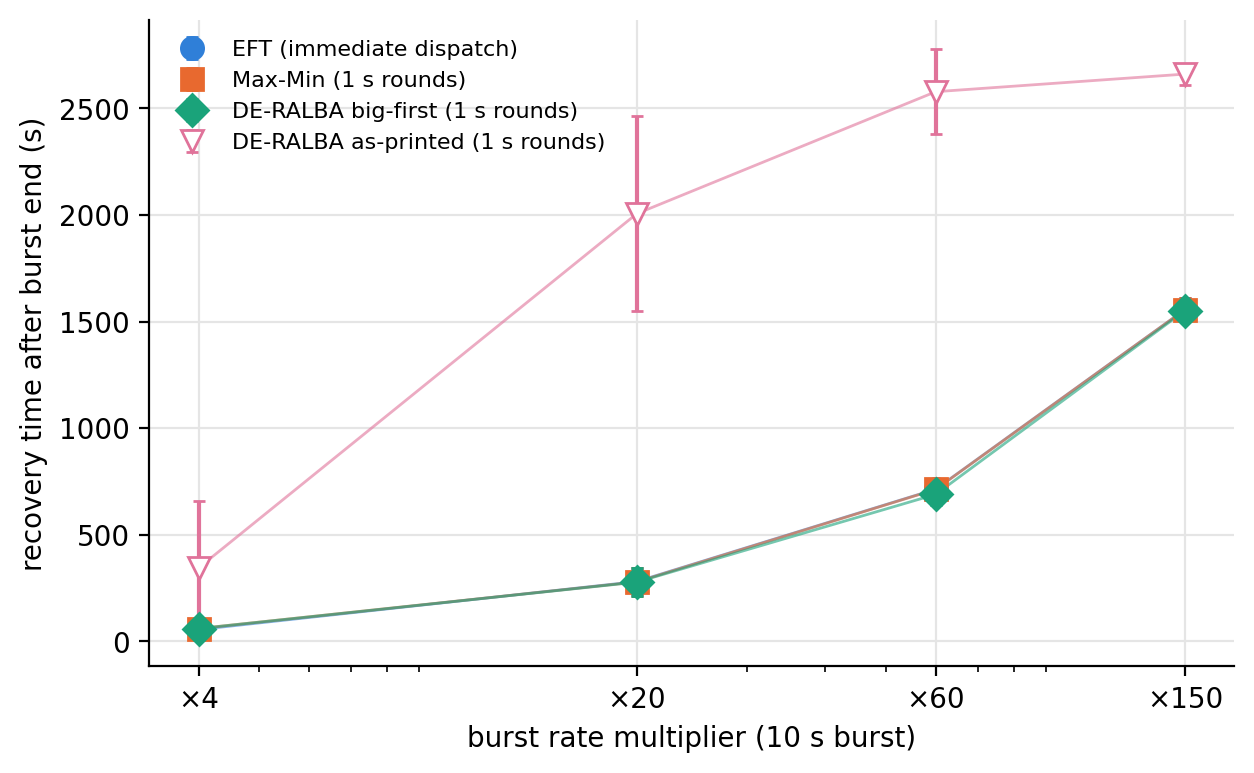
\includegraphics[width=0.75\textwidth]{figures_v2/fig6_recovery.png}
\caption{Recovery time after the end of the burst as a function of burst size (mean and 95\% CI). Hollow markers indicate that at least one seed was censored, so the mean is a lower bound.}\label{fig:recovery}
\end{figure}

Recovery time grows with burst size for every algorithm. For EFT, Dynamic Max-Min and DE-RALBA big-first it rises from about 55--60 s at $4\times$ to about 280 s, 690--715 s and 1,550 s at $20\times$, $60\times$ and $150\times$, and the curves nearly coincide. DE-RALBA as-printed recovers far more slowly (about 345 s at $4\times$, 2,000 s at $20\times$ and over 2,500 s at $60\times$ and $150\times$). Its values are lower bounds because some seeds had not recovered by the last arrival: 1 of 30 at $4\times$, 6 at $20\times$, 3 at $60\times$ and 28 at $150\times$.

\subsection{Effect of the scheduling interval}
At $\rho = 0.5$ and $0.8$, makespan is very similar at both intervals and the 5 s configurations have slightly higher average response times. At $150\times$ the effect is mixed: DE-RALBA-BF with 5 s rounds has lower average and p95 response time than with 1 s rounds, while Dynamic Max-Min with 5 s rounds has a higher average and p95 response time than with 1 s rounds. Figure~\ref{fig:share} helps explain this: panel (a) shows the fraction of cloudlets placed by the share step rather than the EFT step, and panel (b) the mean number of cloudlets per non-empty round.

\begin{figure}[h]
\centering
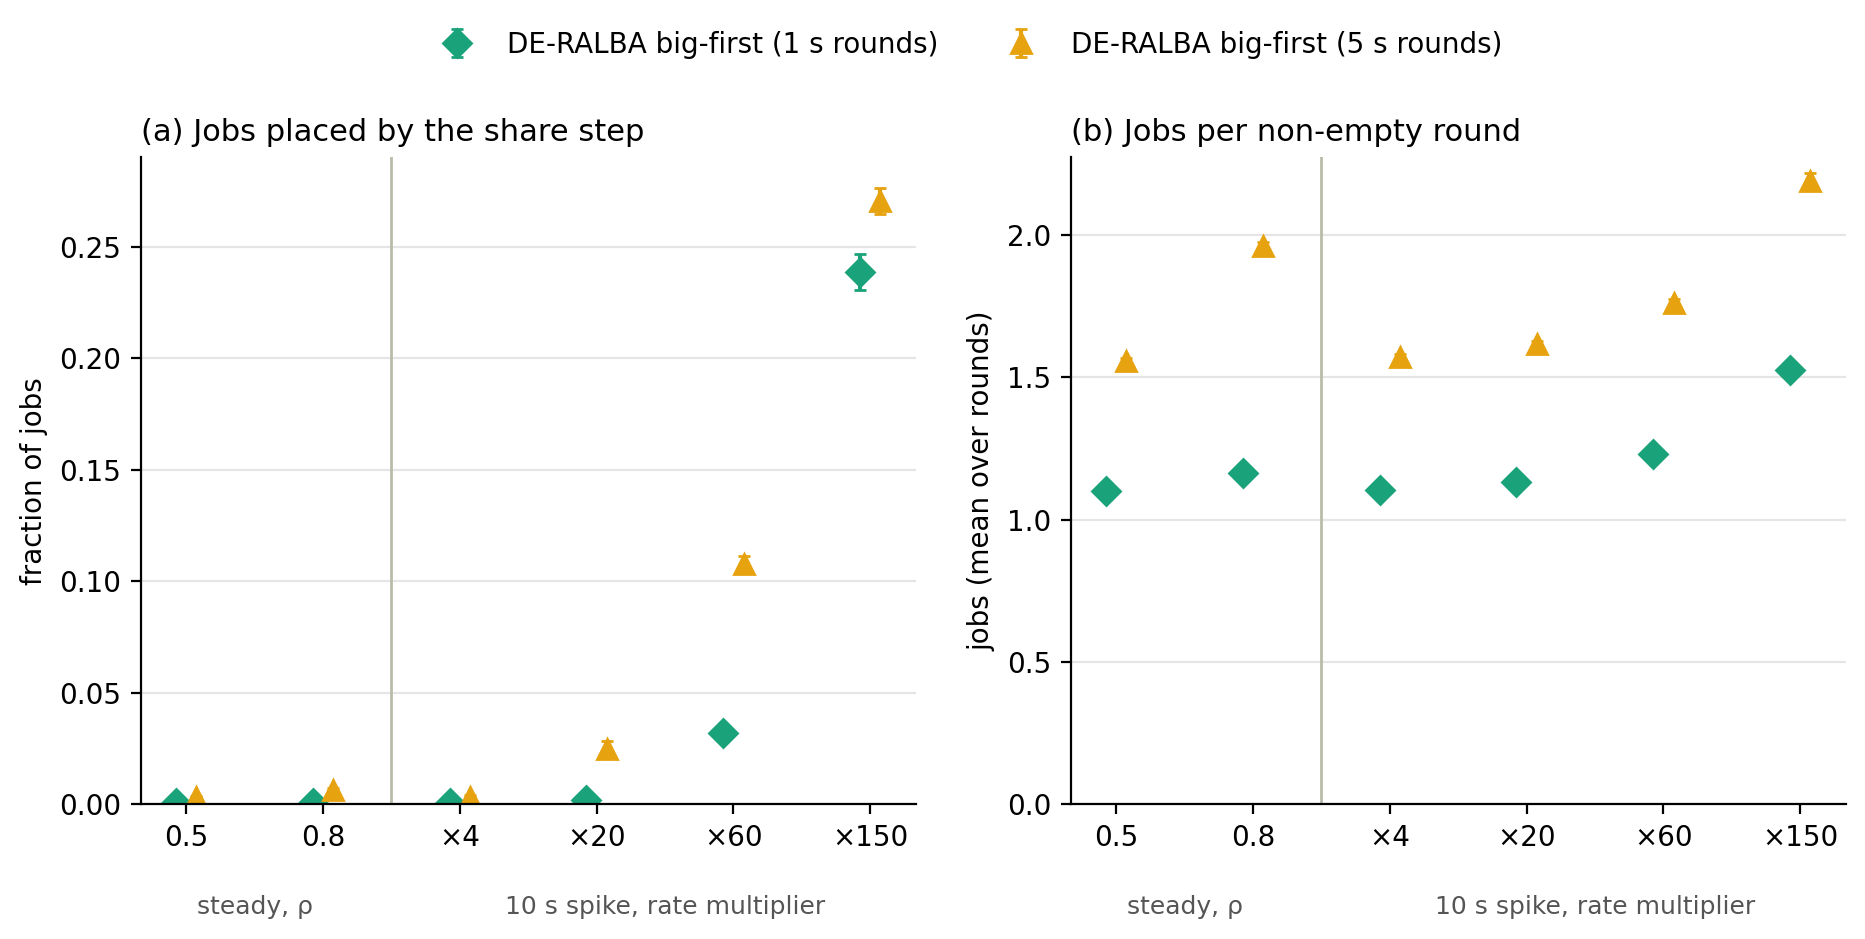
\includegraphics[width=\textwidth]{figures_v2/fig7_share_step.png}
\caption{Use of the share step by DE-RALBA big-first with 1 s and 5 s rounds: (a) fraction of cloudlets placed by the share step; (b) mean number of cloudlets per non-empty round.}\label{fig:share}
\end{figure}

With 1 s rounds, a non-empty round holds only about 1.1--1.5 cloudlets on average, and the share step places almost no cloudlets until the $60\times$ and $150\times$ bursts (about 3\% and 24\%). With 5 s rounds, rounds hold about 1.6--2.2 cloudlets and the share step places about 11\% of cloudlets at $60\times$ and 27\% at $150\times$. The share-based mechanism therefore matters mainly when many cloudlets accumulate in one round, which happens only under intense bursts or with longer intervals; elsewhere DE-RALBA largely behaves like EFT, consistent with its similarity to EFT and Dynamic Max-Min.

\subsection{Effect of the Big-First modification}
At $\rho = 0.5$ and $0.8$, DE-RALBA-LIT and DE-RALBA-BF give almost identical makespan, ARUR and response times. At $150\times$, DE-RALBA-BF with 1 s rounds is slightly lower than DE-RALBA-LIT in makespan and in average, p95 and maximum response time, but with 5 s rounds it is slightly higher in average and p95 response time. The differences are small and change sign with the interval, so the results do not establish a consistent benefit of Big-First.

\subsection{Effect of idle-VM reallocation}
DE-RALBA-BF and DE-RALBA-BF-NOREB differ only in whether idle-VM reallocation is enabled, so their per-seed differences isolate its effect (Table~\ref{tab:ablation} and Fig.~\ref{fig:ablation}).

\begin{table}[h]
\caption{Paired differences DE-RALBA-BF minus DE-RALBA-BF-NOREB (mean and 95\% CI over 30 seeds, in seconds). Negative values mean that reallocation helps. Recovery is defined only for burst scenarios.}\label{tab:ablation}
\centering
\fontsize{6.2pt}{7.6pt}\selectfont
\setlength{\tabcolsep}{1.5pt}
\begin{tabular}{llcccc}
\toprule
Scenario & Interval & Mean RT & p95 RT & Makespan & Recovery \\
\midrule
Steady $\rho=0.5$ & 1 s & $-0.06\ [-0.10, -0.02]$ & $-0.90\ [-2.86, +1.05]$ & $+0.46\ [-0.69, +1.60]$ & --- \\
 & 5 s & $-0.40\ [-0.51, -0.29]$ & $-9.09\ [-14.08, -4.09]$ & $+0.80\ [-2.10, +3.71]$ & --- \\
Steady $\rho=0.8$ & 1 s & $-0.27\ [-0.43, -0.11]$ & $-0.86\ [-2.08, +0.36]$ & $+0.60\ [-5.33, +6.53]$ & --- \\
 & 5 s & $-1.19\ [-1.48, -0.89]$ & $-4.22\ [-6.84, -1.61]$ & $-0.12\ [-9.60, +9.35]$ & --- \\
$4\times$ & 1 s & $-0.12\ [-0.20, -0.04]$ & $-4.16\ [-9.00, +0.68]$ & $-0.52\ [-3.41, +2.38]$ & $0.00\ [0.00, 0.00]$ \\
 & 5 s & $-0.53\ [-0.65, -0.40]$ & $-9.65\ [-15.22, -4.08]$ & $-2.61\ [-6.31, +1.09]$ & $-2.23\ [-6.32, +1.85]$ \\
$20\times$ & 1 s & $-0.30\ [-0.40, -0.20]$ & $-3.50\ [-6.16, -0.84]$ & $-0.56\ [-4.68, +3.56]$ & $-0.40\ [-0.77, -0.03]$ \\
 & 5 s & $-1.62\ [-1.85, -1.38]$ & $-13.66\ [-18.29, -9.03]$ & $-0.86\ [-4.10, +2.39]$ & $-49.57\ [-76.39, -22.75]$ \\
$60\times$ & 1 s & $-1.02\ [-1.20, -0.84]$ & $-4.64\ [-5.99, -3.28]$ & $+0.37\ [-3.27, +4.00]$ & $-23.10\ [-41.22, -4.98]$ \\
 & 5 s & $-1.45\ [-1.74, -1.15]$ & $-6.75\ [-8.85, -4.65]$ & $+0.61\ [-3.74, +4.96]$ & $-24.40\ [-40.67, -8.13]$ \\
$150\times$ & 1 s & $-0.92\ [-1.15, -0.68]$ & $-6.17\ [-8.35, -3.99]$ & $+1.48\ [-3.84, +6.79]$ & $-9.77\ [-26.15, +6.62]$ \\
 & 5 s & $-0.48\ [-0.75, -0.22]$ & $+0.11\ [-0.77, +0.98]$ & $+4.51\ [-1.33, +10.34]$ & $-1.63\ [-5.58, +2.32]$ \\
\bottomrule
\end{tabular}
\end{table}

\begin{figure}[h]
\centering
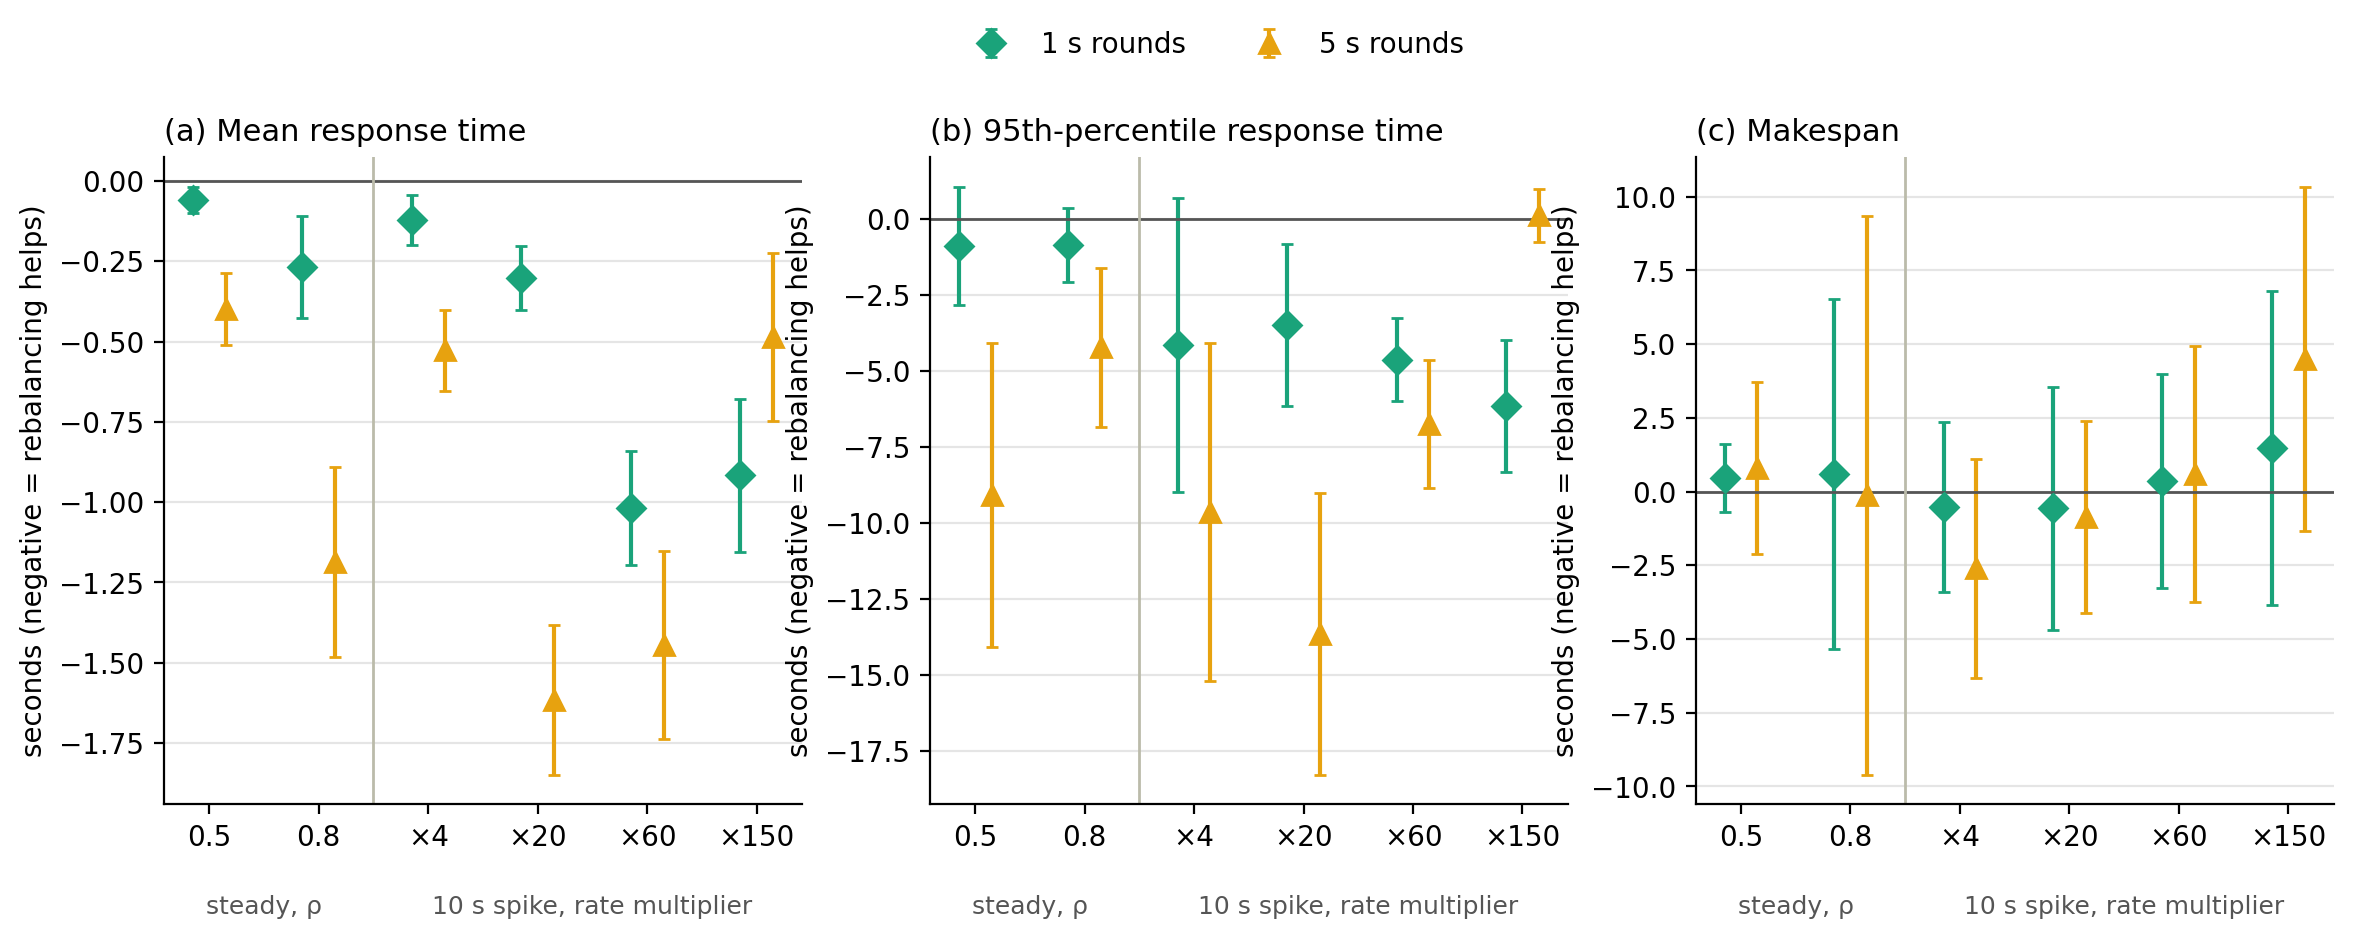
\includegraphics[width=\textwidth]{figures_v2/fig8_rebalancing_ablation.png}
\caption{Paired effect of idle-VM reallocation (DE-RALBA-BF minus DE-RALBA-BF-NOREB) on mean response time (a), 95th-percentile response time (b) and makespan (c), with 95\% confidence intervals. Negative values mean that reallocation helps.}\label{fig:ablation}
\end{figure}

Reallocation reduces the mean response time in all twelve combinations of scenario and interval; the confidence interval excludes zero in every case, although the reductions are small (0.06--1.62 s). It reduces the p95 response time in 11 of 12 combinations, by up to 13.7 s ($20\times$, 5 s), with the confidence interval excluding zero in eight. It shortens recovery significantly at $20\times$ (by 0.4 s with 1 s rounds and 49.6 s with 5 s rounds) and at $60\times$ (both intervals, by about 23--24 s). For makespan, the confidence interval includes zero in all twelve combinations, so reallocation has no measurable effect on makespan. At $150\times$ with 5 s rounds all VMs stay busy for a long time, idle VMs are rare, and reallocation has almost no effect.

\subsection{Summary of findings}
First, RR performs substantially worse than all other evaluated algorithms in every scenario, because its cyclic allocation ignores differences in VM capacity and cloudlet size. Second, EFT, Dynamic Max-Min and the corrected DE-RALBA variants have similar makespan in all scenarios and similar response times up to the $60\times$ burst; at $150\times$ the response-time differences are larger and depend on the scheduling interval. The corrected variants are therefore competitive but not consistently superior. Third, DE-RALBA-AUTHOR-ASIS has higher makespan and response times and much slower recovery. Fourth, Big-First produces only small differences whose sign depends on the interval. Fifth, idle-VM reallocation consistently reduces mean response time, often reduces tail response time and recovery time, and does not change makespan. Finally, longer rounds contain more cloudlets and the share step places more of them, but the 5 s interval does not consistently outperform the 1 s interval.

%======================================================================
\section{Discussion}\label{sec:discussion}
%======================================================================

\subsection{Overall scheduling performance (RQ1)}
Under steady workloads, EFT, Dynamic Max-Min and the corrected DE-RALBA variants give similar makespan and ARUR (Fig.~\ref{fig:mkarur}), so share-based allocation can match established approaches under the tested conditions. Under bursts, differences appear mainly in response time rather than makespan. At $150\times$, makespan (about 4,000 s) and recovery time (about 1,550 s) are similar for EFT, Dynamic Max-Min and the corrected variants, yet EFT has the lowest mean response time and big-first with 1 s rounds is about 18 s slower (Fig.~\ref{fig:paired}). Similar makespan therefore does not imply similar response times. RR performs substantially worse in every scenario, which confirms the importance of considering capacity and estimated completion time on heterogeneous resources.

\subsection{Contribution of the share-based allocation process (RQ2)}
The share-based process gives faster VMs larger proportional shares. In the reported scenarios it produces makespan close to EFT and Dynamic Max-Min, but it does not improve response times: at $150\times$, EFT has a lower mean response time than DE-RALBA-LIT and DE-RALBA-BF. Figure~\ref{fig:share} offers a possible explanation. With 1 s rounds the share step places almost no cloudlets until the $60\times$ and $150\times$ bursts, so DE-RALBA usually behaves like EFT, and the response-time gap appears at the intensities where the share step is used substantially. A possible reason is that the proportional targets of the share step override the earliest-finish placement for individual cloudlets. This is an interpretation, not a proven cause, and per-decision analysis would be needed to confirm it.

\subsection{Big-First and idle-VM reallocation (RQ2)}
Big-First differs little from DE-RALBA-LIT, and the direction of the difference changes with the interval, so the results do not establish a consistent improvement; the effect may depend on the job-size distribution, VM capacities and arrival pattern. Idle-VM reallocation, by contrast, has a consistent effect: it reduces waiting time without changing makespan. It helps most at moderate bursts with 5 s rounds, when more cloudlets wait in queues and idle VMs appear while others are still loaded. It should therefore be understood as a response-time and recovery mechanism rather than a makespan optimisation.

\subsection{Effect of scheduling decision intervals (RQ3)}
A shorter interval allows more frequent decisions, whereas a longer one lets more cloudlets accumulate but adds waiting delay. Makespan and ARUR differ little between 1 s and 5 s, and 5 s rounds have slightly higher average response times under steady load. At $150\times$, DE-RALBA-BF with 5 s rounds has lower mean and p95 response times than with 1 s rounds and is about 14 s faster in mean than Dynamic Max-Min with 5 s rounds. Five-second rounds hold more cloudlets and the share step places a larger fraction of them (about 27\% against 24\% at $150\times$), which may explain why the 1 s disadvantage does not appear in the same way. No interval is universally better.

\subsection{Interpretation of the authors' released implementation}
DE-RALBA-AUTHOR-ASIS has higher makespan and response times than the corrected variants and much slower recovery after the bursts. This is not proof that the published algorithm is incorrect: a description, pseudocode and released code need not lead to identical behaviour, and the interpretation of ambiguous steps can change outcomes. The ready-time update in the released code, which inflates the projected completion times of busy VMs, is a plausible cause of the poor EFT decisions under heavy load. The study therefore documents the variants separately.

\subsection{Implications for evaluating bursty workloads}
Algorithms should be evaluated under more than one arrival pattern, and makespan alone can hide differences in response time and tail behaviour, as at $150\times$ \cite{dean2013tail}. Evaluations should combine makespan with response time, tail response time and recovery time, and using the same seeds across algorithms supports paired comparison and reproducibility.

%======================================================================
\section{Limitations and Threats to Validity}\label{sec:limits}
%======================================================================

\subsection{Simulation-based evaluation}
The cloudlet execution was computed by a queue model of CloudSim Plus space-shared VMs, validated against CloudSim Plus 8.5.7 on four 100-cloudlet schedules but not on every configuration. Neither engine models network delays, storage bottlenecks, virtualisation overhead, hardware failures or variation in resource availability, and reallocated cloudlets are assumed to move without cost. No deployment on a public cloud or evaluation with production traces was performed. The results are therefore simulation-based evidence, not proof of production performance.

\subsection{Workload and infrastructure scope}
The study used one 100-cloudlet GoCJ instance, Poisson arrivals with a single 10-second burst, and one configuration of 50 heterogeneous VMs (52,500 MIPS). Other job-size distributions, repeated or irregular bursts, real arrival traces \cite{reiss2012heterogeneity}, and other VM capacities may change the relative performance of the algorithms, so the findings should not be generalised without further experiments.

\subsection{Algorithm interpretation and implementation differences}
Implementing DE-RALBA required interpreting parts of the original description; for example, this study uses the minimum in the EFT equation instead of the printed maximum, and it uses its own status accounting in place of Eqs.~(\ref{eq:exec})--(\ref{eq:ready}). The corrected interpretation and the port of the released implementation are not identical, since status updates, cloudlet selection and idle-VM reallocation differ. The results are therefore not a direct reproduction of every internal behaviour of the original implementation.

\subsection{Big-First, intervals and metrics}
Big-First is an experimental modification introduced here, not part of DE-RALBA, and its effect needs testing with other job-size distributions and infrastructures. Only 1 s and 5 s intervals are analysed in this paper. The metrics leave out energy, cost, network traffic, memory, I/O, fault tolerance and SLA violations. ARUR is based on VM busy times and is not a time-averaged CPU utilisation, and the recovery time depends on the chosen threshold and observation horizon; for DE-RALBA-AUTHOR-ASIS, censored seeds make its recovery values lower bounds.

\subsection{Statistical scope}
Each configuration used 30 paired seeds, which reduces variation from generated workloads. Separate confidence intervals around means do not by themselves establish significant differences between algorithms. Paired confidence intervals are reported for the reallocation ablation (Table~\ref{tab:ablation}) and for selected comparisons with the baselines (Fig.~\ref{fig:paired}); they are not adjusted for multiple comparisons.

%======================================================================
\section{Conclusion and Future Work}\label{sec:conclusion}
%======================================================================
This study evaluated DE-RALBA under steady and bursty workloads in a simulated heterogeneous cloud, comparing it with Round Robin, EFT and Dynamic Max-Min and examining several DE-RALBA variants and two scheduling intervals.

Round Robin was clearly the worst performer, with much higher makespan and response times. The corrected DE-RALBA variants were competitive with EFT and Dynamic Max-Min but not consistently superior. At the $150\times$ burst, makespan (about 4,000 s) and recovery time (about 1,550 s) were similar across EFT, Dynamic Max-Min and the corrected variants, while response times diverged, so makespan alone concealed burst-related differences. With 1 s rounds, non-empty rounds contained only about 1.1--1.5 cloudlets on average and the share step placed very few cloudlets until the $60\times$ and $150\times$ bursts, which may explain why the corrected variants often resembled EFT. Idle-VM reallocation reduced mean response time in every tested configuration and often reduced tail response time and recovery time, without changing makespan. Big-First produced only small differences whose direction depended on the interval.

The port of the authors' released implementation had higher makespan and response times and much slower recovery; at $150\times$, 28 of 30 seeds had not recovered by the observation limit. This result characterises the current port and its implementation choices, not the intrinsic quality of the published algorithm. The study does not evaluate DRALBA, PSSLB or PSSELB and makes no claim about the original paper's reported gains against those baselines.

Future work can (1) use more workload datasets and arrival patterns, such as repeated or irregular bursts and other job-size distributions; (2) vary the infrastructure in VM capacities and heterogeneity; (3) evaluate further scheduling intervals and their overhead; (4) include energy, cost, network and I/O performance, and SLA violations; (5) extend the paired analysis to all algorithm pairs with a multiple-comparison adjustment; and (6) evaluate the algorithms in a real cloud environment or a detailed testbed.

\section*{Declarations}
\begin{itemize}
    \item \textbf{Funding}: No external funding was received for this study.
    \item \textbf{Competing interests}: The authors declare that they have no competing interests.
    \item \textbf{Data and code availability}: The source code, workload files, raw per-run results (\texttt{results/summary.csv}) and figures are available at \url{\repourl} \cite{spikelb2026repo}.
    \item \textbf{Third-party material}: Figures~\ref{fig:arch} and~\ref{fig:flow} are reproduced from Hussain et al.\ \cite{hussain2025deralba} under the Creative Commons Attribution 4.0 licence.
    \item \textbf{Author contributions}: All authors contributed equally to the study design, implementation, experiments, analysis and writing.
    \item \textbf{Use of AI tools}: An AI assistant was used to cross-check the reported values against the experiment output files, to regenerate figures from those files, to format the paper in the Springer LaTeX template, and to draft parts of the text (the abstract, parts of the related work, the validation and idle-VM reallocation analyses, and some discussion paragraphs). The authors designed and ran the experiments, reviewed all AI-assisted text, and take full responsibility for the content.
    \item \textbf{Student details}: Kunal Kashyap (2024UIT3126), Anshal (2024UIT3090) and Parna Hembram (2024UIT3115), Department of Information Technology, NSUT.
\end{itemize}

\bibliography{sn-bibliography}

\end{document}
